\documentclass[sigconf]{acmart}

%\settopmatter{printacmref=false} % Removes citation information below abstract
%\renewcommand\footnotetextcopyrightpermission[1]{} % removes footnote with conference information in first column
\pagestyle{plain} % removes running headers
%\usepackage{enumitem}
\usepackage{subcaption}
\usepackage{verbatim}

\usepackage{multirow}
\usepackage{hyperref}
\usepackage{xspace}
\usepackage{caption}

\newcommand{\AG}[1]{\textcolor{red}{#1}}
\newcommand{\TD}[1]{\textcolor{blue}{#1}}
\setcopyright{rightsretained}


\usepackage{amsmath}

\usepackage[inline]{enumitem}

\newenvironment{tightitemize}%
	 {\begin{list}{$\bullet$}{%
 		\setlength{\leftmargin}{10pt}
        \setlength{\itemsep}{0pt}%
        \setlength{\parsep}{0pt}%
        \setlength{\topsep}{0pt}%
        \setlength{\parskip}{0pt}%
        }%
 }%
{\end{list}}

\newcounter{tecounter}
\newenvironment{tightenumerate}%
 {\begin{list}{\arabic{tecounter}.}{%
 		\usecounter{tecounter}
 		\setlength{\leftmargin}{10pt}
        \setlength{\itemsep}{0pt}%
        \setlength{\parsep}{0pt}%
        \setlength{\topsep}{0pt}%
        \setlength{\parskip}{0pt}%
        }%
 }%
{\end{list}}%


\begin{document}

\title{CoMerge: Toward Efficient Data Placement in Shared Heterogeneous Memory Systems}

\author{Thaleia Dimitra Doudali}
\affiliation{%
\institution{Georgia Institute of Technology}
}
\email{thdoudali@gatech.edu} 

\author{Ada Gavrilovska}
\affiliation{%
\institution{Georgia Institute of Technology}
}
\email{ada@cc.gatech.edu} 



% Use the following at camera-ready time to suppress page numbers.
% Comment it out when you first submit the paper for review.
\thispagestyle{empty}
\pagenumbering{gobble}


\begin{abstract}
Emerging systems with heterogeneous memory components demand new mechanisms and policies for spanning applications' data 
across the complex memory substrate. This is particularly important for data-intensive scientific or analytics applications, 
demanding both large memory capacity and fast access speeds, which can only be satisfied by embracing memory heterogeneity. 
Current approaches advocated in research are based on detailed full-application profiles, and while they show promise with respect 
to their effectiveness, their utility can be limited when considering multi-tenant environments, that need to support collocation and dynamic activity of different applications.
As a step toward extending the current state-of-the-art, we propose {\it CoMerge}, a memory-sharing rather than partitioning technique, that prioritizes allocations of performance-critical data 
across collocated applications, with respect to their overall sensitivity to changes in memory latency and bandwidth. 
\end{abstract}


\begin{CCSXML}
<ccs2012>
<concept>
<concept_id>10010583.10010786.10010787</concept_id>
<concept_desc>Hardware~Analysis and design of emerging devices and systems</concept_desc>
<concept_significance>300</concept_significance>
</concept>
<concept>
<concept_id>10010583.10010786.10010787.10010788</concept_id>
<concept_desc>Hardware~Emerging architectures</concept_desc>
<concept_significance>300</concept_significance>
</concept>
<concept>
<concept_id>10010583.10010786.10010787.10010791</concept_id>
<concept_desc>Hardware~Emerging tools and methodologies</concept_desc>
<concept_significance>300</concept_significance>
</concept>
</ccs2012>
\end{CCSXML}

\ccsdesc[300]{Hardware~Analysis and design of emerging devices and systems}
\ccsdesc[300]{Hardware~Emerging architectures}
\ccsdesc[300]{Hardware~Emerging tools and methodologies}

\keywords{Hybrid Memory Management, Shared Heterogeneous Memory Systems, Data Tiering}

\copyrightyear{2017} 
\acmYear{2017} 
\setcopyright{acmcopyright}
\acmConference{MEMSYS 2017}{October 2--5, 2017}{Alexandria, VA, USA}\acmPrice{15.00}\acmDOI{10.1145/3132402.3132418}
\acmISBN{978-1-4503-5335-9/17/10}

\maketitle

\section{Introduction}
\label{sec:intro}

Data-intensive applications pose demands for memory capacity and speeds that cannot be addressed with DRAM, given its cost and scaling issues. As a result, a plethora of new memory technologies have emerged -- from fast, but small-capacity High Bandwidth Memory (HBM), to much slower and larger non-volatile memories (NVM). 
Thus, future systems will couple small portions of ``fast'' memory (DRAM or HBM) with larger amounts of ``slow'' memory (NVMs, or off-chip DRAM relative to on-chip memory), creating a heterogeneous memory substrate. 

In such hybrid memory systems, data-intensive applications, that require significant amounts of memory capacity, will end up spanning their dataset across both fast and slow memory components. Careful management of the dataset mapping is necessary in order to maximize the utility of the available fast memory, and achieve application performance that approaches a limit equivalent to an all-fast-memory mapping. 

There has already been progress on developing support for data placement, i.e., tiering, and for dynamic data management across memory components in a hybrid memory system. Most of the hardware or system-level solutions are focused on improving over current heterogeneity-unaware techniques, however there continues to be a significant gap relative to the ideal all-fast-memory executions~\cite{sudarsun:isca17,Chou:Batman}. To bridge this gap, new interfaces~\cite{memkind} and application profiling methodologies~\cite{Dulloor:tiering,Shen:dataplacer,Pena:knapsack} are being proposed. The goal of these approaches is to allow application developers to perform {\em a-priori} detailed profiling of the application's use of its different data structures, and based on some notion of cost, establish partial ordering of the data structures (or regions of memory). This ordering is then used to prioritize the placement of ``high priority'' data structures to the available fast memory. 


For instance, Dulloor et al.~\cite{Dulloor:tiering} explore the data placement problem for data-intensive cloud applications such as data stores and graph applications. They 
observe that the frequency of accesses to a data structure is not sufficient to define the cost by itself. Additional knowledge of the access pattern 
(sequential, random, pointer chasing) is necessary, as it varies the effective access latency in modern superscalar out-of-order processors. Also, 
they observe that the density of accesses may not be uniform across the whole data structure size, thus they break the cost calculations on a memory region granularity. 
In this way, they can place parts of a data structure in a memory component due to restricted available capacity. 
Similarly, Du Shen et al.~\cite{Shen:dataplacer} perform array-centric cost calculations based on the same observations, using the array size and access distribution, and adding cache reuse tracking for data locality classification. 
In both cases, the authors are able to establish an ordering of the data structure regions such that the resulting placement in the available fast memory leads to improvements in application performance and efficiency. 
Pe\~{n}a and Balaji take a different approach by mapping the placement arrangement to the multiple knapsack problem, where the knapsacks are the different memory components of a certain capacity, 
the weight of the data structures is their size and the value is the number of the load cache misses that they incur~\cite{Pena:knapsack}. Using a small set of HPC applications, they too are able to obtain data layouts that improve performance. 


While these efforts are successful in establishing memory allocations which lead to performance gains, they make the assumption that one application can make exclusive use of all the available fast memory. 
Given the fact that datacenter and exascale systems are shared environments, there needs to be a solution that accounts for different applications running simultaneously, sharing resources 
and competing for fast memory allocations. Existing solutions can be directly applied in multi-tenant environments, using static memory partitioning schemas. 
%static because they require offline profiling. 
However, such techniques trade-off resourse to application fairness. 
For example, a resource-fair schema will divide the available memory into equal portions for every collocated application, whereas an application-fair layout will split memory into sizes proportional to the 
overall workload's memory footprint. Additionally, they still do not account for the overall priority of an application against another. The priority can be directly associated with the applications QoS requirements, or it can be established based on its
sensitivity against execution over slow memory. More specifically, if an application benefits more than others from using fast memory, it should be given priority in allocating data in fast memory. 
Overall, there are many parameters that need to be addressed, in order to be able to provide performance gains across co-running applications.




%While these efforts are successful in establishing memory allocations which lead to performance gains, we argue that more work is needed to develop efficient methodology for deciding how to span application data across hybrid memories. 
%The utility of {\em a-priori} profiling of full applications is limited when dealing with dynamic workloads, or when workloads are collocated in shared multi-tenant environments. The profiling complexity increases with application complexity, and it is unclear what effect it will have on the portability of the applications and the development cycle. The expectation that developers would engage in careful analysis of the ideal layout of their data for each workload, is not scalable. Even for domains where ``hero'' programmers are the norm -- such as the HPC domain -- current plans for next generation systems exhibit sufficient differences in the configurations of fast vs.~slow memory~\cite{ascr:facilities}, that programmer-guided placement methods will limit the portability of the codes. 
%Furthermore, these prior efforts already illustrate some diversity of the factors that guide the decision process --  frequency and density of memory accesses, the cache reuse and the access pattern, data sizes, etc. -- thus begging the question which one(s) are the right ones to consider. 
%On the other hand, the use of purely low-level, application-agnostic metrics, relies purely on modeling in a complex parameter space comprising multitude of systems-software- and hardware-generated events, where it may be difficult to gain confidence in the derived heuristics. In addition, it does not take advantage of higher-level information that may be available at the application or runtime level. 
%In summary, it is necessary to establish more practical approaches to how application state should be distributed and re-distributed across the memory substrate in a dynamic manner.  
%.....

%In addition, these insights can provide for more rapid decisions on how to best leverage slow memory and leave space in the fast memory for more important data structures -- ones which have higher {\em benefit factor}. Such notion of a benefit factor, associated with entire data structures or memory regions, could be useful in establishing future policies for sharing heterogeneous memories across collocated applications. 
%Motivated by these observations, we investigate the opportunities to reduce or eliminate the reliance on full application profiles in future data management solutions for hybrid memory systems. 

Motivated by these requirements, we investigate the opportunity to enrich the existing data tiering solutions, in order to facilitate efficient data placement in shared environments. 
We pursue this specifically targeting a wide range of data-intensive scientific application kernels, with goals of providing insights relevant to the HPC community looking to revamp its systems software stacks and toolchains in preparation for the next generation pre-exascale systems with heterogeneous memories, such as ORNL's Summit and LLNL's Sierra. 
%ANL's Aurora.  -- Aurora as proposed is getting killed, rumors are already out. what will go there instead will be something very different with specialized accelerators but not clear if interesting in terms of memory. 
We make the following initial observations:

\begin{tightenumerate}
\item Applications can have varying degrees of sensitivity when accessing data allocated in slower memory components. These can very from high and medium to low and even non-existing. 
The case of non-sensitive workloads is particularly important as it eliminates the need for offline profiling and data tiering, 
at least not beyond established benefits related to increasing the aggregate system bandwidth~\cite{Chou:Batman}.  
\item The contribution of the applications' data structures to the overall performance shows great variability as well. There are cases where computational kernels have dominant 
data objects, whose allocation to the fast memory is absolutely crucial to the overall application performance. 
\item The above two observations apply across single as well as multi-threaded application kernels.
\item Static memory partitioning schemas fail to leverage the full potential of the existing solutions and performance gains, due to possible capacity restrictions and placement cost calculations that are 
agnostic to the collocation impact. 
\end{tightenumerate}


In fact, the utility of {\em a-priori} profiling of full applications
%, followed by static partitioning or memory-sharing schemas, 
%\TD{at this point we haven't said anything for memory sharing techniques so far, so maybe we should just say static partitioning schemas?}
is limited when dealing with dynamic workloads, particularly when workloads are collocated in shared multi-tenant environments. The profiling complexity increases with application complexity, and it is unclear what effect it will have on the portability of the applications and the development cycle. The expectation that developers would engage in careful analysis of the ideal layout of their data for each workload, is not scalable. Even for domains where ``hero'' programmers are the norm -- such as the HPC domain -- current plans for next generation systems exhibit sufficient differences in the configurations of fast vs.~slow memory~\cite{ascr:facilities}, that programmer-guided placement methods will limit the portability of the codes. 
By focusing on key application components, that define a big part of the application performance and overall need of fast memory, 
developers, or future toolchains and dynamic resource managers, can make certain placement decisions more rapidly, potentially expanding additional monitoring and analysis cycles on a much smaller portion of the applications' memory accesses. 


Based on these observations, we propose {\bf CoMerge} -- a memory-sharing technique that makes decisions on a data structure level granularity and prioritizes fast memory allocations of performance-critical data across 
the different applications with respect to their degree of sensitivity to slow memory. 
CoMerge relies on the novel metric of {\it co-benefit}, that is able to capture the data structure-level contribution to application's performance, as well as the sensitivity of the overall workload to execution over slower memory components.
%We make the following interesting observations that complement the existing work on generating guidelines for intelligent data placement, 
%which can be integrated into a future systems-level solution. 
%\begin{tightenumerate}
%\item The use of slow memory does not necessarily degrade the performance of every single application. In such cases, 
%there is no need to perform cost calculations and explicit placement, at least not beyond established benefits related to increasing the aggregate system bandwidth~\cite{Chou:Batman}.  
%\item In the partial ordering of the data structures, there is a non-linear degradation of the ``weight'' of the data structures' contribution to the application's performance sensitivity to memory. 
%In fact, we observe that only a small portion of the full set of application data structures truly contribute to the performance sensitivity to memory characteristics.  
%\item At the level of the application and its algorithms, there is generally fairly clear intuition into which data structures should be weighted higher when considering their prioritization to faster memory. 
%\end{tightenumerate}
%These observations are important to be captured as we seek improvements in the data management infrastructure for emerging heterogenous memory systems. 
Experimental analysis with the Polybench benchmark suite and several CORAL mini apps, show that CoMerge is able to improve performance across all collocated applications, as well as provide high utilization of the shared fast memory.

\section{Experimental Methodology}
\label{sec:methodology}

\noindent{\bf Testbed. }
All analysis presented in this paper are based on experimental data gathered on a
testbed emulating 
a heterogeneous memory environment. 
The testbed consists of 
a 12-core dual-socket Intel Xeon platform, with two 4 GB DDR3
nodes, and 12 MB shared Last Level Cache. We emulate ``slow memory'', referred to as
SlowMem from here on,  by adjusting
the latency and bandwidth of one of the DRAM sockets, as done in prior
research~\cite{Kannan:pVM, sudarsun:isca17}.
More specifically, we apply thermal throttling to reduce the socket's bandwidth, as well as increase the effective access latency, 
thus experimenting with various combinations which result in slower access to the specific socket.
%In this way, we are able to emulate up to 9x lower bandwidth and 5x longer latency, when accessing the SlowMem. 
We refer to the baseline memory performance based on the other DRAM memory node as FastMem. 
Table~\ref{tab:throttle} summarizes the latency and bandwidth values, as well as the corresponding approximate 
factors of bandwidth reduction and latency increase.\\

\begin{table}[t]
%\vspace{-0.2in}
\centering
%\footnotesize
\begin{tabular}{|p{1.6cm}|p{0.6cm}|p{0.6cm}|p{0.8cm}|p{0.7cm}|p{0.7cm}|p{0.7cm}|}
\hline
Factor & B:1 L:1 & B:1 L:2 & B:0.5 L:3 & B:0.25 L:2.5 & B:0.2 L:5 & B:0.15 L:5\\ \hline
Latency (ns) & 67 & 131 	& 197 		& 174 		& 310 	& 300 \\ \hline
BW (GB/s) & 11.7 & 11.7 	& 4.9 		& 2.8 		& 2.2 	& 1.7\\ \hline
\end{tabular}
\caption{Testbed Bandwidth and Latency values for DRAM (B:1 L:1) and emulated NVM (B:x L:y) of 
x times reduced bandwidth and y times increased latency.}
\label{tab:throttle}
\vspace{-0.3in}
\end{table}

\noindent{\bf Benchmarks. } 
We base part of our analysis on the Polybench/C benchmark suite \cite{polybench}, as it provides a big range of representative scientific applications, from linear algebra kernels and solvers, 
to stencil computations and data mining algorithms. It consists of simple kernels with clear marking, that are being widely used as building components in HPC applications. 
The original version of the benchmark suite does not support
multi-threaded execution, but there exist modified versions suitable
for multicores, GPUs and accelerator environments \cite{polybench:gpu}. For
brevity, we focus
the current discussion on the observations made with the
single-threaded versions of the benchmarks, as they already
stress the applications' sensitivity to the memory subsystem. 

Additionally, we choose three of the `skeleton benchmarks' in the
CORAL suite of mini apps \cite{coral:suite}: XSBench \cite{Tramm:wy},
CLOMP \cite{Bronevetsky:2008} and STREAM \cite{stream}. These are
benchmarks of significantly bigger size  (in terms of lines of code)
and they have access patterns that are representative of HPC
applications. We deploy their OpenMP version, thus extending our
analysis to multi-threaded applications, as they may have different
behavior when running over heterogeneous memory subsystems. The
experiments are done configuring these applications to run as many
threads as the available cores on the Node, which is 12 in our
testbed. Brief description of these benchmarks is provided in Section ~\ref{sec:placement}.\\

\noindent{\bf Methodology. } The analyses presented in the paper are
grouped in two categories. The first group, in Section ~\ref{sec:sensitivity}, describes the overall
sensitivity analysis for the target applications, as a function of the
different memory parameters emulated on our testbed. 
The second group 
focuses on a subset of applications and performs a deep-dive analysis 
of how select application components (i.e., data structures)
contribute to its performance sensitivity (in
Section~\ref{sec:placement}), and how do collocation and memory
partitioning techniques impact the overall performance across
applications (Section~\ref{sec:collocation}). For this second part 
we configure SlowMem to be accessed with 0.2x the bandwidth and 5x
the latency of FastMem. Also, for the collocation analysis we further restrict the available FastMem from 4 GB down to e.g. 3 GB or 2 GB, so that the aggregate workload sizes exceed the capacity. The SlowMem is always fixed to 4 GB capacity.
We use the Linux NUMA API to  
explicitly allocate memory in FastMem and SlowMem. All application's datasets are not exceeding the available memory on the NUMA sockets, thus they do not result in virtual paging. Finally, the application processes have the same standard execution priority on the Linux platform.




\section{Sensitivity Analysis}
\label{sec:analysis}
\subsection{Overall Application Sensitivity}
\label{sec:sensitivity}

\begin{figure}[t]
\centering
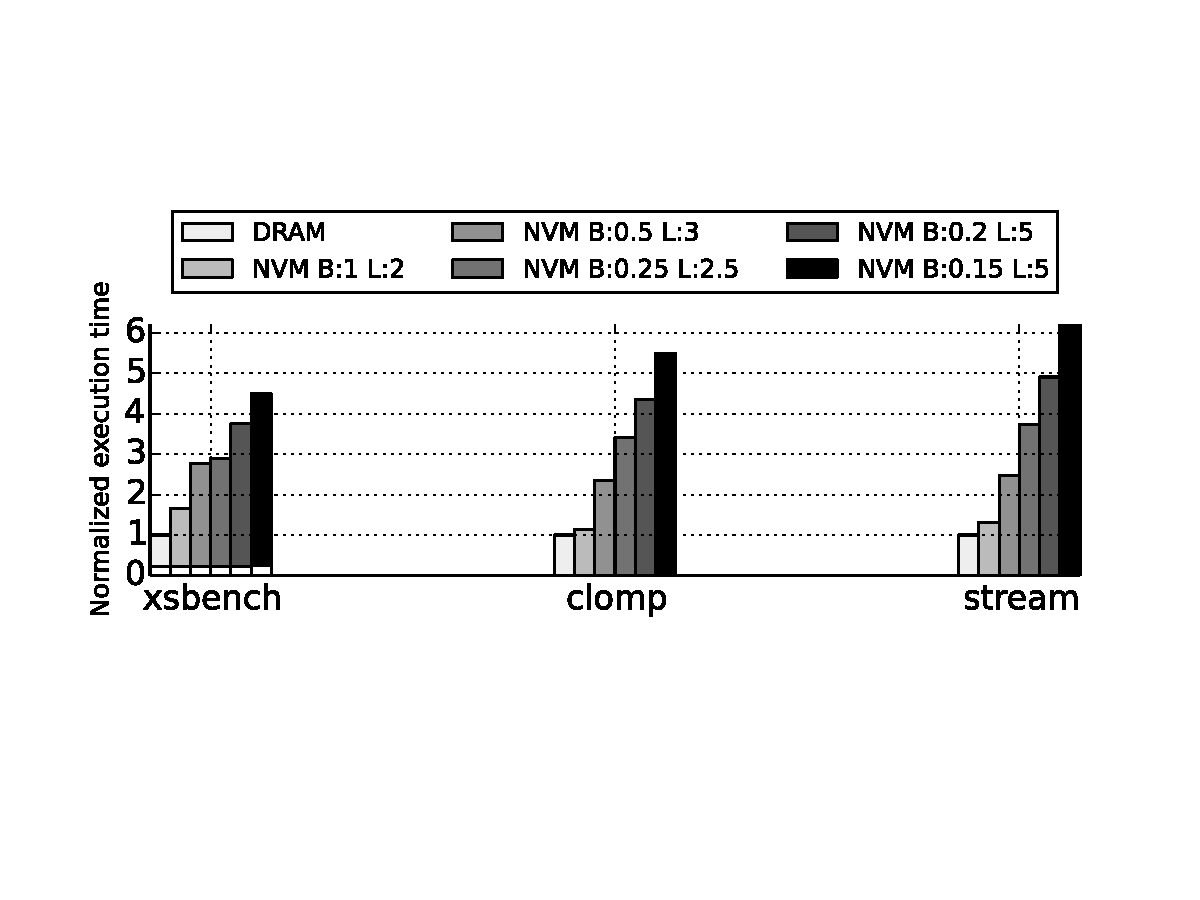
\includegraphics[width=\columnwidth]{figures/coral_throttle.pdf}
\caption{Performance slowdown across three CORAL benchmarks, normalized to `all-in-DRAM' execution. The white bottom part in XSBench shows the corresponding runtime of its initialization phase.}
\label{fig:coral_throttle}
\vspace{-0.2in}
\end{figure}

\begin{figure*}[t]
\centering
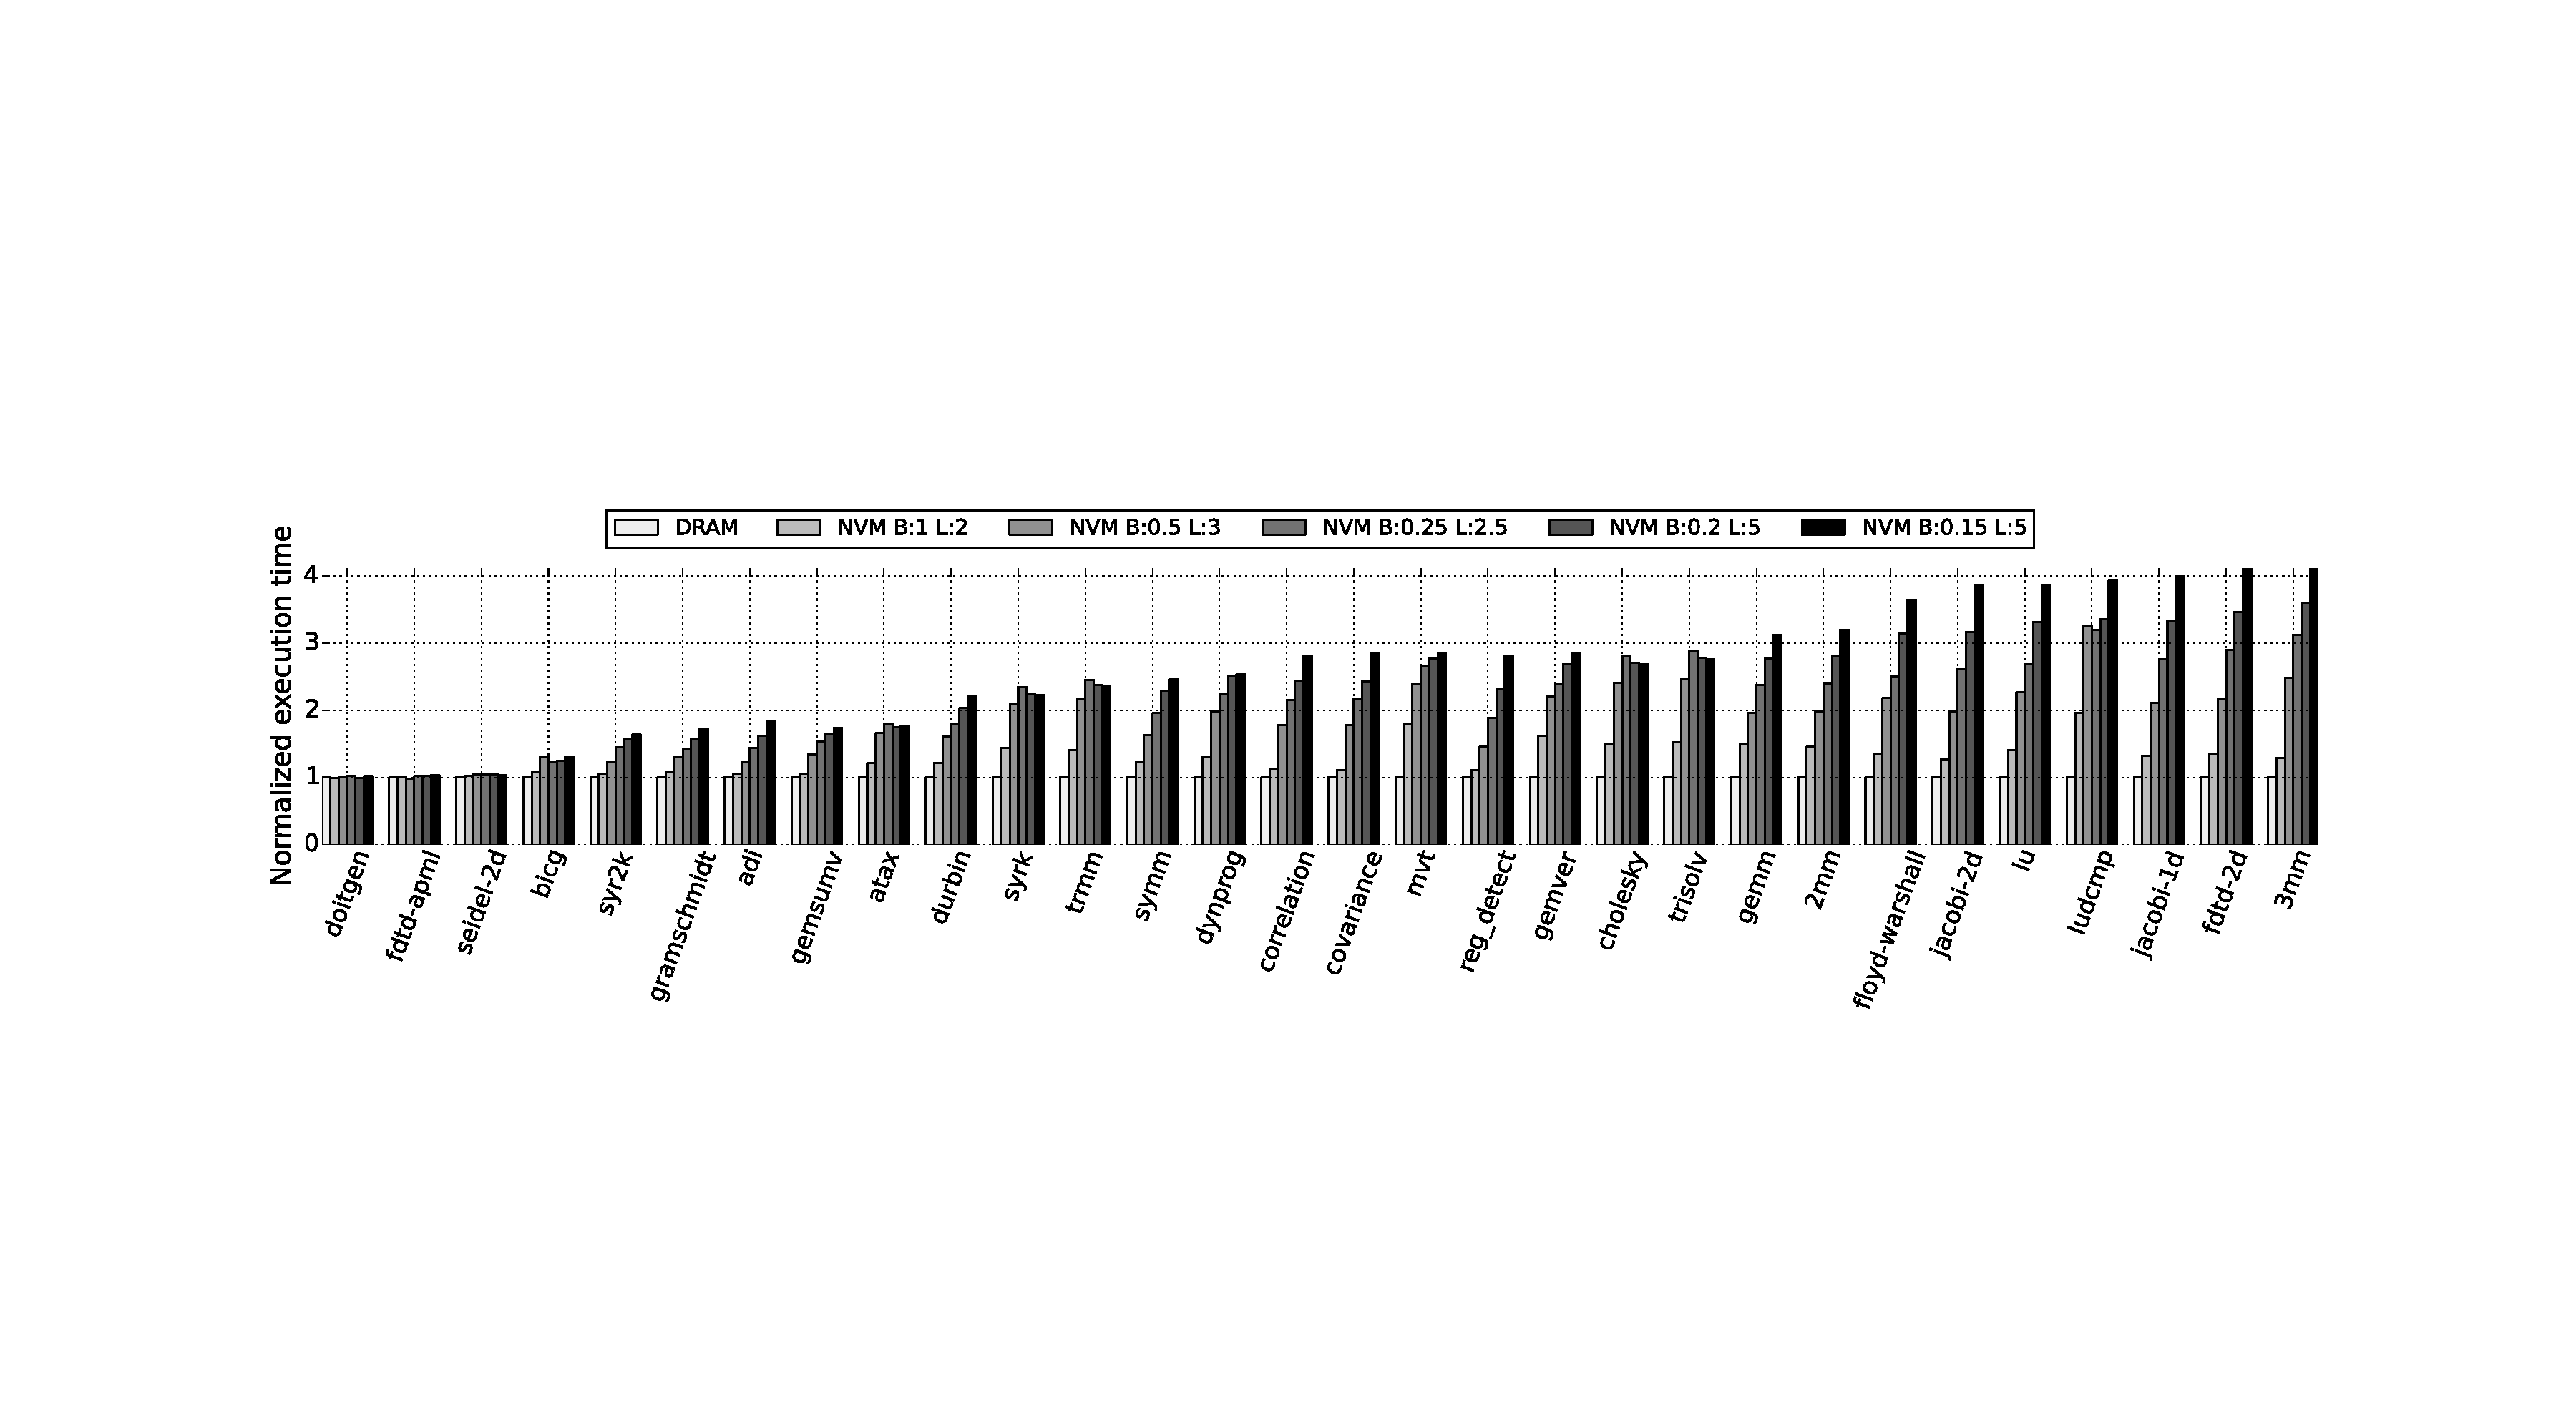
\includegraphics[width=\textwidth]{figures/polybench_throttle.pdf}
\caption{Performance slowdown across Polybench/C, normalized to `all-in-DRAM' execution.}
\label{fig:poly_throttle}
\end{figure*}

\vspace{0.6ex}
%\subsubsection
\noindent{\bf\em CORAL Experiments}
\vspace{0.3ex}

\noindent Figure ~\ref{fig:coral_throttle} shows the run time slowdown of the CORAL benchmarks when all data is allocated in SlowMem, for different combinations of bandwidth and latency, normalized to the baseline where all data lives in FastMem. We observe 
that all three applications are highly sensitive to SlowMem data allocations and accesses,  because the execution time increases when memory accesses are getting even more throttled. In the case of emulated NVM with 0.15 times less bandwidth and 5 times bigger latency, we see a 4x-6x slowdown from FastMem execution, which is very significant. 

In particular, the XSBench kernel consists of two discrete phases: the initialization phase which is run by a single thread in the beginning of execution, and the actual computation phase which is done by all 12 OpenMP threads in parallel. 
%\AG{this was very hard to see, it took me a while to realize what you were pointing to. you can use color for the bars to make it more visible, or make it all white so it stands out more explicitly. }
The white bottom part in XSBench in Figure~\ref{fig:coral_throttle} shows the total XSBench slowdown, when the computation phase is configured to have few iterations, such that the initialization phase dominates the runtime. In this case, we see that the overall application run time is not sensitive to execution over slower memory components. 



\vspace{2.0ex}

%\subsubsection
\noindent{\bf\em Polybench Experiments}
\vspace{0.3ex}

\noindent Similarly, Figure~\ref{fig:poly_throttle} shows the performance slowdown in the execution time of the Polybench suite in a setup where all data is in the available SlowMem  
(for different levels of throttled bandwidth and latency) compared to 
a baseline configuration where all data fits in FastMem.  We observe that there are kernels that 
execute up to 4x times slower in an SlowMem-only system, 
as well as others that do not get affected at all by the slower memory environment. We can classify the kernels into four distinct levels of 
sensitivity, which correspond to the degree of performance slowdown they incur, due to SlowMem-only memory accesses, as summarized in Table ~\ref{tbl:poly_class}. \\

\begin{table}[t]
\centering
{%\footnotesize
    \begin{tabular}{|p{1.4cm}|p{5.5cm}|p{0.6cm}|} \hline
	\textbf{Sensitivity \newline level} & \textbf{Kernels} & \textbf{Total} \\ \hline \hline
	None & doitgen, fdtd-apml, seidel-2d & 3/33 \\ \hline
	Low  & bicg, syr2k, gramschmidt, adi, gemsumv, atax & 6/33 \\ \hline
	Medium & durbin, syrk, trmm, symm, dynprog, correlation, covariance, mvt, reg\_detect, gemver, cholesky, trisolv & 12/33 \\ \hline
	High & gemm, 2mm, floyd-warshall, jacobi-2d, lu, ludcmp, jacobi-1d, fdtd-2d, 3mm, XSBench, CLOMP, STREAM & 12/33 \\ \hline
    \end{tabular}
}
\caption{Sensitivity classification across the 30 Polybench and 3 CORAL Benchmarks.}
\label{tbl:poly_class}
\vspace{-0.3in}
\end{table}


\noindent{\bf\em Takeaways}\\
The observation that not all applications (or some of their phases) are equally sensitive, when accessing slower memory components, can enable even more sophisticated decisions in data tiering solutions.
For example, non sensitive kernels can leverage the presence of SlowMem, allocating their entire dataset there, eliminating any need for offline profiling and finer granularity data placement decisions. 
Also, they further facilitate possible application co-running senarios, by leaving more available FastMem space for other workloads, that may have a higher sensitivity degree to SlowMem. 
More broadly, the overall sensitivity of an application is an extra parameter that needs to be taken into account when thinking about resource partitioning in shared environments. It can be used as an 
overall priority factor, when determining the amount of FastMem that each application can use, as we describe in Section ~\ref{sec:collocation}. Finally, the degree of sensitivity is also 
important to be captured for applications that have to respect Quality of Service (QoS) guarantees. It can determine the level of extra performance tuning needed to provide similar services in heterogeneous 
memory systems, compared to current DRAM-only environments.

%We can classify the kernels into three distinct categories of 
%sensitivity levels in the presence of slower memory:

%\begin{tightitemize}
%\item {\it Bandwidth sensitive}: the execution time grows linearly with the different levels of bandwidth throttling.
%\item {\it Latency sensitive}: the execution time grows linearly and shows a knee when latency does not further increase.
%\item {\it Non sensitive}: the execution time is constant across the different levels of latency and bandwidth throttling.
%\end{tightitemize}

%\begin{table}[t]
%\centering
%{\footnotesize
%    \begin{tabular}{|p{1.4cm}|p{5.5cm}|p{0.6cm}|} \hline
%		\textbf{Sensitivity \newline factor} & \textbf{Kernels} & \textbf{Total} \\ \hline \hline
%		Bandwidth & syr2k, gramschmidt, adi, gemsumv, durbin, symm, dynprog, correlation, covariance, mvt, reg\_detect, 
%					gemver, gemm, 2mm, floyd-warshall, jacobi-2d, lu, ludcmp, jacobi-1d, fdtd-2d, 3mm & 21/30 \\ \hline
%		Latency & bicg, atax, syrk, trmm, cholesky, trisolv & 6/30 \\ \hline
%		None & doitgen, fdtd-apml, seidel-2d & 3/30 \\ \hline
%    \end{tabular}
%}
%\caption{Sensitivity classification across Polybench/C.}
%\label{tbl:poly_class}
%\vspace{-0.3in}
%\end{table}

%\begin{figure*}[t]
%\centering

%    \begin{subfigure}[b]{\textwidth}
%	\includegraphics[width=\textwidth]{figures/miss_mpki.eps}
	%\end{subfigure}
    %\begin{subfigure}[b]{\textwidth}
	%\includegraphics[width=\textwidth]{figures/pref_loads.eps}
	%\end{subfigure}
    %\begin{subfigure}[b]{\textwidth}
	%\includegraphics[width=\textwidth]{figures/ipc.eps}
	%\end{subfigure}
%\caption{Performance metrics across Polybench/C.}
%\label{fig:poly_cache}
%\end{figure*}

%able~\ref{tbl:poly_class} sumarizes the classification of the different benchmarks into one of the above categories. Although the majority of kernels is bandwidth sensitive, there are few that are impacted  
%ostly by latency and others that do not get affected by any factor. 

%We next investigate whether the sensitivity of the kernels to slow memory can be easily characterized using low-level memory usage metrics such as cache use, workload size, prefetching effectiveness, etc. 
%the reasons that determine the level of sensitivity of the kernels to slow memory, looking deeper into 
%the effects of cache use, workload size and prefetching. 
%Figure~\ref{fig:poly_cache} shows the MPKI, LLC miss ratio, the number of total memory loads, the LLC prefetch miss ratio, the CPI and IPC for every benchmark in Polybench. 
%We use the Linux profiling tool \textit{perf} to extract these values for the same size of the workload used in the results shown in Figure~\ref{fig:poly_throttle}.

%Regarding the non-sensitive kernels, both \textit{doitgen} and \textit{seidel-2d} have very low MPKI values indicating this is not a memory-bound workload -- hense this classification is expected. 
%In the case of \textit{doitgen} the LLC miss ratio is 0.1\%, so the workload access pattern is cache-friendly.
%In contrast, \textit{seidel-2d} has poor cache locality with a very high LLC miss ratio, but the number of total memory load requests is low, less than 200 millions, thus 
%computation can hide the effects of not efficient cache use. For the last non-sensitive kernel, \textit{fdtd-apml}, the MPKI is not very low, rather quite larger than other kernels which do 
%exhibit sensitivity to SlowMem. However, \textit{fdtd-apml} issues a very small amount of memory load requests, around 9 million, enabling overlapped computation to 
%counter against the very poor cache locality. 

%In the case of latency sensitive kernels, the LLC miss ratio is very high, around 90\% across all of them. However, the MPKI shows great variability, as it can be as low as 1.21 in the 
%\textit{trmm} kernel or as big as 16.65 in the \textit{trisolv} kernel. A high value of MPKI usually indicates a memory intensive workload, but it is possible for a low MPKI value 
%to increase the sensitivity to latency. This is the case for \textit{trmm}, where even though the MPKI is really low, and the low CPI suggests a compute intensive workload, the number of 
%memory load requests is so big, close to 1,500 million, that ends up dominating and converting the workload to memory intensive. Additionally, 
%the access pattern of \textit{trmm} (Triangular matrix multiply) is such that doesn't allow good cache locality, as the LLC miss rate is  94.96\%, further enhancing the 
%sensitivity to latency.

%Bandwidth sensitivity is the most common one across Polybench and it can incur 1.5x up to 4x slowdown for 9x bandwidth throttling level. 
%There is a group of kernels that make very good use of the cache and prefetching having very low miss ratios, 
%such as \textit{2mm}, \textit{gemm}, \textit{gemver}, \textit{mvt}, \textit{symm}, \textit{durbin}, \textit{gramschmidt} and \textit{reg\_detect}. 
%In all these kernels the maximum slowdown will be less than 3x, indicating that good cache reuse limits the number of memory requests and 
%doesn't get impacted by the throttled bandwidth. The MPKI of these specific kernels again varies, it can be as low as 0.025 in \textit{reg\_detect} or 
%as big as 24.85 in \textit{durbin}. In the case of \textit{reg\_detect} the number of memory loads is only 500,000 and even though MPKI is so low, 
%the throttled bandwidth does impact the overall execution time.

%Thaleia: I want to sum up the observations, as well as give directions as to what metric we should choose to understand in which sensitivity level the workload belongs.
%In conclusion, we first observe that workloads which are compute intensive can benefit form the use of cache or superscalar out-of-order execution, 
%becoming resistant to slower memory accesses. In such cases, the LLC miss ratio can be misleading whereas the MPKI and workload size (number of memory load requests) can better hint the 
%potential for a non sensitive type of workload. Next, regarding the latency sensitive kernels, we notice that the LLC miss ratio is consistently high indicating potential sensitivity, 
%whereas the MPKI alone can be insufficient, as a really low MPKI value in combination with high number of load requests converts the workload to memory intensive. Finally, 
%in the case of bandwidth sensitive there are quite few kernels with very good data locality, suggesting that good cache reuse can hint sensitivity to bandwidth, and there can even be workloads 
%with very low values of MPKI and memory load requests, that get affected when running over slower memory as there is limited bandwidth they can benefit from.  \\

%\noindent{\em Summary of observations. } In summary, there are complex relationships among the application-sensitivity and these low-level events, without a clear correlation. Applying sophisticated learning methods will likely reveal greater insights, but even then building scalable models purely on low level metrics alone may be too costly, or even ineffective. 


\subsection{Data Structure Sensitivity}
\label{sec:placement}


\begin{table*}[t]
\centering
{\footnotesize
	\begin{subtable}{0.31\linewidth}
    \begin{tabular}{|p{1cm}|p{0.8cm}|p{0.55cm}|p{0.55cm}|p{0.75cm}|} \hline
	FastMem alloc & Time & Benefit & Co-benefit & Size \\\hline \hline	
	All & 35.37 s & 1 & 3 & 1 GB\\\hline
	{\ttfamily nuclide} & 42.58 s & 0.9 & 2.7 & 30 MB \\\hline
	{\ttfamily energy} & 102.38 s & 0.14 & 0.42 & 970 MB \\\hline
      None & 113.17 s & 0 & 0 & 0 \\\hline
    \end{tabular}
	\subcaption{XSBench (high)}
	\label{tbl:tiering_xsbench}
	\end{subtable}
}
{\footnotesize
	\begin{subtable}{0.31\linewidth}
    \begin{tabular}{|p{1cm}|p{0.8cm}|p{0.55cm}|p{0.55cm}|p{0.85cm}|} \hline
	FastMem alloc & Time & Benefit & Co-benefit & Size \\\hline \hline	
	All & 49.3 s & 1 & 3 & 1.5 GB\\\hline
	{\ttfamily parts} & 160.1 s & 0.019 & 0.057 & 250 MB \\\hline
	{\ttfamily zones} & 49.4 s & 0.99 & 2.97 & 1250 MB \\\hline
      None & 162.2 s & 0 & 0 & 0 \\\hline
    \end{tabular}
	\subcaption{CLOMP (high)}
	\label{tbl:tiering_clomp}
	\end{subtable}
}
{\footnotesize
	\begin{subtable}{0.31\linewidth}
    \begin{tabular}{|p{1cm}|p{0.8cm}|p{0.55cm}|p{0.55cm}|p{0.75cm}|} \hline
	FastMem alloc & Time & Benefit & Co-benefit & Size \\\hline \hline	
	All & 28.83 s & 1 & 3 & 1.6 GB\\\hline
	{\ttfamily a} & 75.38 s & 0.4 & 1.2 & 534 MB \\\hline
	{\ttfamily b} & 75.53 s & 0.39 & 1.17 & 534 MB \\\hline
	{\ttfamily }c & 61.19 s & 0.59 & 1.77 & 534 MB \\\hline
      None & 106.55 s & 0 & 0 & 0 \\\hline
    \end{tabular}
	\subcaption{STREAM (high)}
	\label{tbl:tiering_stream}
	\end{subtable}
}

{\footnotesize
	\begin{subtable}{0.3\linewidth}
    \begin{tabular}{|p{1cm}|p{0.8cm}|p{0.55cm}|p{0.55cm}|p{0.75cm}|} \hline
	FastMem alloc & Time & Benefit & Co-benefit & Size \\\hline \hline
	All & 29.45 s &  1 & 0 & 1 GB \\\hline 
	{\ttfamily C4} & 29.68 s & 0.81 & 0 & 1 MB \\\hline
	{\ttfamily sum} & 29.9 s & 0.63 & 0 & 498 MB \\\hline
	{\ttfamily }A & 30.5 s & 0.15 & 0 & 498 MB \\\hline
	None & 30.69 s & 0 & 0 & 0 \\\hline
    \end{tabular}
	\subcaption{doitgen (none)}
	\label{tbl:tiering_doitgen}
	\end{subtable}
}
{\footnotesize
	\begin{subtable}{0.3\linewidth}
    \begin{tabular}{|p{1cm}|p{0.8cm}|p{0.55cm}|p{0.55cm}|p{0.75cm}|} \hline
	FastMem alloc & Time & Benefit & Co-benefit & Size \\\hline \hline	
	All & 116.86 s & 1 & 1 & 1.5GB \\\hline
	{\ttfamily X} & 136.38 s & 0.62 & 0.62 & 500 MB \\\hline
	{\ttfamily B} & 141.17 s & 0.53 & 0.53 & 500 MB \\\hline
	{\ttfamily A} & 150.47 s & 0.34 & 0.34 & 500 MB \\\hline
     None & 168.15 s & 0 & 0 & 0 \\\hline
    \end{tabular}
	\subcaption{adi (low)}
	\label{tbl:tiering_adi}
	\end{subtable}
}
{\footnotesize
	\begin{subtable}{0.3\linewidth}
    \begin{tabular}{|p{1cm}|p{0.8cm}|p{0.55cm}|p{0.55cm}|p{0.75cm}|} \hline
	FastMem alloc & Time & Benefit & Co-benefit & Size \\\hline \hline	
	All & 56.44 s & 1 & 2 & 250 MB \\\hline
	{\ttfamily B} & 56.98 s & 0.99 & 1.98 & 125 MB \\\hline
	{\ttfamily A} & 130.25 s & 0.04 & 0.08 & 125 MB \\\hline
      None & 133.05 s & 0 & 0 & 0 \\\hline
    \end{tabular}
	\subcaption{trmm (medium)}
	\label{tbl:tiering_trmm}
	\end{subtable}
}
{\footnotesize
	\begin{subtable}{0.33\linewidth}
    \begin{tabular}{|p{1cm}|p{0.8cm}|p{0.55cm}|p{0.55cm}|p{0.75cm}|} \hline
	FastMem alloc & Time & Benefit & Co-benefit & Size \\\hline \hline	
	All & 49.55 s & 1 & 3 & 1.5 GB \\\hline
	{\ttfamily hz} & 114.07 s & 0.48 & 1.44 & 500 MB \\\hline
	{\ttfamily ey} & 127.91 s & 0.37 & 1.11 & 500 MB \\\hline
	{\ttfamily ex} & 138.83 s & 0.29 & 0.87 & 500 MB \\\hline
      None & 174.58 s & 0 & 0 & 0 \\\hline
    \end{tabular}
	\subcaption{fdtd-2d (high)}
	\label{tbl:tiering_fdtd}
	\end{subtable}
}
{\footnotesize
	\begin{subtable}{0.33\linewidth}
    \begin{tabular}{|p{1cm}|p{0.8cm}|p{0.55cm}|p{0.55cm}|p{0.75cm}|} \hline
	FastMem alloc & Time & Benefit & Co-benefit & Size \\\hline \hline	
	All & 28.67 s & 1 & 3 & 1 GB\\\hline
	{\ttfamily A} & 59.64 s & 0.61 & 1.83 & 500 MB \\\hline
	{\ttfamily B} & 62.52 s & 0.58 & 1.74 & 500 MB \\\hline
      None & 109.7 s & 0 & 0 & 0 \\\hline
    \end{tabular}
	\subcaption{jacobi-2d (high)}
	\label{tbl:tiering_jacobi}
	\end{subtable}
}

\caption{Execution time in data tiering. Application sensitivity classification in parentheses.}
\label{tbl:tiering}
\vspace{-1ex}
\end{table*}

Next, we analyse the application sensitivity to data tiering across FastMem and SlowMem, using the testbed described in Section~\ref{sec:methodology}. 
We choose a few representative kernels from Polybench Suite across different sensitivity groups, as well as the three CORAL benchmarks, and look deeper into the algorithm that they implement, as well as the primary data structures they define. 
Then, we run each benchmark with different placement configurations. More
specifically, using the Linux NUMA API we place into FastMem one data structure at a time, allocating the rest in SlowMem, and measure the overall 
execution time of the application. 
This type of data tiering allows us to capture the benefit of 
placing a particular data object into FastMem, by observing the
difference in execution time between the two distinct configurations,
where all data is placed either in FastMem or SlowMem. 

We define the {\em benefit} of placing data object $O$ into FastMem as follows, where t is the corresponding application execution time, F and S are the execution times when all objects are in FastMem and SlowMem, respectively.
\[Benefit(O) = \frac{t(O)-S}{F-S}\]
The benefit factor can range between 0, which is the all-in-SlowMem configuration, to 1 being the all-in-FastMem configuration.
A high benefit factor close to 1, indicates that the data structure $O$
significantly contributes to the application's memory sensitivity, and
should get high priority in getting allocated in FastMem. Thus, using these benefit factor values for the different data objects of an
application, we are able to define a partial ordering of them, in a
similar way done by the related work described in Section~\ref{sec:intro}. Table~\ref{tbl:tiering} summarizes the execution times and benefit calculations across kernels  
from different sensitivity levels. 
More specifically, the first row of each table represents the best case scenario, where all data objects are allocated in FastMem, therefore the benefit factor is 1 and the size reflects the total 
memory footprint of the application. Similarly, the last row corresponds to the worst case scenario, where all data allocations are serviced from SlowMem, forcing a zero benefit factor. The middle rows 
highlight the execution time of the application, when only one particular object is allocated in FastMem, and the performance benefit the application gets, when this object is accessed through FastMem. 
The notion of co-benefit factor will be introduced in Section~\ref{subsec:merge}.\\

%\subsubsection
\vspace{0.6ex}
\noindent{\bf\em CORAL Experiments}
\vspace{0.3ex} 

\noindent The bechmarks from the CORAL suite are all very sensitive to execution over SlowMem, thus we do a deep-dive analysis for each one.\\

\noindent{\bf XSBench.} XSBench is mini app that simulates the  most computationally intensive part of the Monte Carlo transport algorithm, which is the calculation of macroscopic neutron cross-sections~\cite{Tramm:wy}. As per the official CORAL description, the purpose of XSBench is to stress the memory subsystem of a single node. The user can define the number of nuclides and gridpoints per nuclide, as well as the number of lookups of cross-section data that will be performed. The first two define the dataset size and the last one the length of the computation. The mini app consists of two discrete phases, the initialization of the data, which is done by the main thread, and the core computation of lookups, which is done in parallel by the number of thread the user configures. If the number of lookups defined is not big enough, then the initialization phase dominates the run time, as we observed in Section~\ref{sec:sensitivity}.  There are two main data structures, the {\ttfamily nuclide grid},
 which holds the matrix of nuclide grid points, and the {\ttfamily energy grid} which holds the corresponding energy values. 

We experiment with 12 threads, 355 nuclides, 2000 grid points per nuclide and 50 million lookups. Table~\ref{tbl:tiering_xsbench} holds the raw values of the total run time (initialization and computation phase), when all data is allocated in FastMem only and SlowMem only, as well as the benefit factors of the individual data structures. We observe that the data structure {\ttfamily energy grid} has only a benefit factor of 0.14 compared to the 0.9 of {\ttfamily nuclide grid}, even though its size is extremely larger, being 970 MB compared to 30 MB. This is due to the fact that accesses to the {\ttfamily nuclide grid} result in a significant number of Last Level Cache misses due to its access pattern, thus the mini app spends a lot of stall cycles waiting to load {\ttfamily nuclide grid} data from memory~\cite{Pena:2016}. 
This is why the application benefits immensely when this object is allocated in FastMem. 
Therefore, we not only see that there may be significant difference in the contribution of the different data structures to the overall application slowdown, but also that this difference may be independent of the size of the object itself. \\

\noindent{\bf CLOMP.} CLOMP is a benchmark designed to capture OpenMP overheads, as well as general threading, NUMA, caching, prefetching and memory latency and bandwidth factors that impact application performance~\cite{Bronevetsky:2008}. There are two main data structures that formulate an unstructured mesh, {\ttfamily parts} and {\ttfamily zones} which correspond to the two dimensions of the mesh.  The computation over the mesh is very basic algebra, so that the result can be verifiable. Essentially, {\ttfamily parts} is a list of pointers to the {\ttfamily zones}, and the computation is done over the {\ttfamily zones}. The benchmark consists of 7 individual sub-tests running one after the other, testing different individual threading overheads. 

We experiment with 12 threads and a mesh of 64000 parts of 640 zones each, where each zone is 32 bytes. 
Table~\ref{tbl:tiering_clomp} shows the overall slowdown of the aggregate execution time of all the 7 tests when all data is allocated in SlowMem, compared to the case where all fits in FastMem. We see that the {\ttfamily parts} list of pointers has trivial benefit factor, something that is expected because it is accessed only as a gateway to the {\ttfamily zones}.  {\ttfamily Zones} is the main data structure where computation is done as it is also reflected in its size. This is the reason why {\ttfamily zones} has benefit factor value almost close to 1. Thus, it is crucial that it is allocated in FastMem, otherwise the impact of using FastMem will be negligible and the application runtime will be as if all data was allocated in SlowMem.\\

\noindent{\bf STREAM.} STREAM is the predominant synthetic benchmark  to measure the bandwidth of a memory node~\cite{stream}. It reports the computation rate (MB/s) and execution time of four distinct kernels over three matrix data structures {\ttfamily a}, {\ttfamily b} and {\ttfamily c}. More specifically, the computation kernel is  \(c = a\) for `copy', \(b = scalar*c\) for `scale', \(c = a + b\) for `add', and \(a = b + scalar*c\) for `triad'.

We experiment with 12 threads and matrix size of 70 million elements each. Table~\ref{tbl:tiering_stream} shows the aggregate runtime of all four kernels when the matrices are allocated in FastMem and the slowdown when all are in SlowMem. The different matrices have similar benefit factor values, with matrix {\ttfamily c} having the higher one, due to the fact that it is accessed across all four kernels, whereas {\ttfamily a} and {\ttfamily b} participate only in three kernels. Therefore, {\ttfamily c} should be prioritized for allocation in FastMem, following {\ttfamily a} and then {\ttfamily b} who have trivial difference in the benefit factor value. \\

%\subsubsection
\vspace{1ex}
\noindent{\bf\em Polybench Experiments}
\vspace{0.3ex}

\noindent Overall, there is great variability in the benefit factor values of the different data objects amongst the various Polybench kernels. We look deeper into what are the algorithm and data structures of the following kernels, which belong in different sensitivity groups. \\

%\AG{make the way you're presenting this consistent with the above. I made a change in the first kernel. }

\noindent{\bf doitgen.} The multiresolution analysis kernel doitgen
uses two 3D matrices {\ttfamily A} and {\ttfamily sum} and one 2D matrix {\ttfamily C4}. The computation can be summarized as $sum = sum + A*C4$. 
Since the kernel is not sensitive to the presence of SlowMem, we see small variability in the execution time for the different tiering configurations, as per Table~\ref{tbl:tiering_doitgen}. 
However, the benefit calculations can still define a partial ordering of {\ttfamily C4 > sum > A}. 
Although {\ttfamily C4} is of trivial size compared to the other data structures, it receives such an amount of accesses that attributes a higher benefit factor than the others.\\

\noindent{\bf adi.} The alternating direction implicit solver kernel uses three two-dimensional matrices of the same size. The mathematical formula is more complex, but it is such that the number of accesses per matrix give a different benefit factor value to each one, ordering them as {\ttfamily X > B > A}, as per Table~\ref{tbl:tiering_adi}. However, as far as the total runtime is concerned, there is no significant difference across the various data tierings, because the kernel has low overall sensitivity to execution over slower memory.\\

\noindent{\bf trmm.} The triangular matrix multiply kernel calculates a triangular matrix multiplication of $B = A*B$, where {\ttfamily A} and {\ttfamily B} are matrices of the same size. The fact that matrix {\ttfamily B} is getting much more read and write accesses than {\ttfamily A}, in combination with 
the irregular access pattern of the triangular multiplication, results in the accesses to matrix {\ttfamily B} being crucial to the overall application performance, as we can see in Table~\ref{tbl:tiering_trmm}. \\

\noindent{\bf fdtd-2d.} The 2D finite different time domain kernel uses three two-dimensional matrices of the same size, which have similar benefit factor values. Overall, the application is very sensitive to slower memory, because every data tiering configuration incurs between 2x-3.5x slowdown from the all-in-FastMem configuration, as per Table~\ref{tbl:tiering_fdtd}, thus intelligent data placement of the different data structures is crucial to performance.\\

\noindent{\bf jacobi-2d.} The 2D jacobi stencil computation kernel uses two two-dimensional arrays {\ttfamily A} and {\ttfamily B} of equal size, in order to solve the $A*x = B$ using the Jacobi method. Both matrices are almost equally important for performance, as their benefit factor values are very similar, according to Table~\ref{tbl:tiering_jacobi}. Also, the kernel overall is very sensitive to slower memory and the benefit factors of the matrices are around 0.5 meaning that placing even one of them in FastMem can mitigate the overall slowdown by 50\%.\\

\noindent{\bf\em Takeaways}
\vspace{0.3ex}

\noindent Overall, we see that there can be high variability in the contribution of each data structure to the application runtime. We capture this contribution into a {\it benefit factor} value. On the one hand, there are kernels whose data objects have similar such values, so allocating any of them in FastMem can mitigate to some degree the slowdown from running the whole application over SlowMem. On the other side, there are kernels where the difference between the benefit factor of the objects is extremely significant and placement of one data structure to FastMem is the only way to mitigate the slowdown from allocating all data in SlowMem. Also, these observations apply to both single as well as multi-threaded applications, highlighting the importance for clever data placement decisions over a broad spectrum of application kernels and algebraic computations. Moving forward, these remarks are especially important to be captured in shared environments, where 
co-existing applications will compete for the available FastMem and sophisticated data tiering solutions are the only way to maximize performance across a group of applications, instead of just one. 

%Since I'm not presenting the Pin numbers, I don't want to mention them at all.
\begin{comment}
Using Pin we get the number of accesses that each data structure incurs. Metrics such as the size, the access pattern, the access frequency and density are used in related work, in order to 
attribute similar notions of cost on a data object granularity. 
In this way, we validate that the definition of cost, that the related
work provides, is correct and indeed reflects on the actual overall
execution time of the application. For brevity we present the
execution times and benefit calculations and not the raw numbers
related to accesses obtained with Pin. 
\end{comment}

%Following is a deep dive analysis of six representative kernels from Polybench/C. 




\begin{comment}

%\paragraph
\noindent{\bf doitgen:} Multiresolution analysis kernel. Non sensitive.\\
The kernel uses two 3D matrices $A$ and $sum$ and one 2D matrix $C4$. The computation can be summarized as $sum = sum + A*C4$. 
Since the kernel is not sensitive to the presence of SlowMem, we see small variability in the execution time for the different tiering configurations. 
However, the benefit calculations can still define a partial ordering of $C4 > sum > A$. This agrees with cost calculations that take into account the access frequency. 
Although $C4$ takes up only 512 KB, it receives a significantly high amount of read requests compared to $sum$, which receives few writes and $A$ which incurs few reads, when each take up 128 MB. 
Thus, both the benefit and cost computations imply that $C4$ should have
higher priority, than $sum$ and $A$, into being allocated in FastMem. 

However, it is important to observe that, in the 
case of non-sensitive kernels, there is no real performance benefit in performing data tiering. Rather, it imposes extra overhead in tracking the required metrics on a 
data structure granularity. Instead, if a kernel is classified as non sensitive the best practice would be to allocate all data in SlowMem, so as to eliminate extra calculations and 
preserve free space in FastMem for other possible co-located sensitive applications.%\\

%\noindent
%\paragraph
{\bf trmm:} Triangular matrix multiply. Latency sensitive.\\
The kernel multiplies the 2D matrices $A$ and $B$ according to the formula $B = alpha*A*B$, where $alpha$ is a constant.
The benefit calculations indicate that there is 0.99 benefit from placing $B$ in FastMem, whereas $A$ incurs only 0.04, defining a priority order of $B>A$. 
This also agrees with cost calculations, which 
take into account the fact that $A$ and $B$ have the same size, same number of reads, but $B$ also incurs writes as it stores the multiplication result. 
The big difference in the benefit value suggests that $A$ can be allocated in SlowMem, not impacting performance, and reducing in half the space needed in FastMem. %\\

%\noindent
%\paragraph
{\bf bicg:} Biconjugate gradient stabilized method, portion of BiCGStab linear solver. Latency sensitive.\\
The kernel uses a 2D matrix $A$ and 1D matrices $p$, $q$, $r$, $s$ to compute $s =s + r*A$ and $q =q + A*p$. 
The benefit values form a partial ordering of $A > s = q > p = r$. This can be justified by the fact that $A$ is significantly big in size (3 GB) and receives most reads and writes, 
whereas the rest data objects are only 156 KB each, receive the same amount of reads, whereas $q$ and $s$ incur additional writes as well.
Therefore, in this particular kernel it is essential to allocate A in FastMem, requiring very big amounts of available capacity, thus making the allocation of the rest data objects 
of total size 624 KB trivial. %\\

%\noindent
%\paragraph
{\bf 2mm:} Two matrix multiplications. Bandwith sensitive.\\
The kernel computation is $tmp = alpha*A*B$ and $D = tmp*C $. It uses an additional $tmp$ matrix to hold the intermediate multiplication of matrices $A$ and $B$. 
The partial ordering derived by the benefit values is $B = C > D = A =
B$. 
%ada: 
%\AG{what about temp, is that relevant?}
This is due to the fact that $B$ and $C$ receive significantly larger number of reads, even though 
all matrices are of the same size. When placing both B and C into FastMem, the benefit is 0.99, indicating that both data objects should be placed in fast. Since there is 
not significant benefit from placing the remaining data structures into FastMem, they can be allocated into SlowMem and reduce the space needed in FastMem more than 2 times.%\\

%\noindent
%\paragraph
{\bf covariance:} Calculation of covariance. Bandwith sensitive.\\
The kernel computes the covariance $cov_{x,y}=\frac{\sum_{i=1}^{N}(x_{i}-\bar{x})(y_{i}-\bar{y})}{N-1}$. 
The input resides in matrix $data$, the mean in matrix $mean$ and the result in matrix $symmat$.
The benefit values formulate an ordering of $data > symmat > mean$. The input matrix $data$ gets a very big amount of reads, compared to the other two matrices, 
thus incurs the biggest benefit value. In contrast, the result matrix $symmat$ even though has the same size as $data$, incurs only a few writes, leading to a trivial benefit value. 
Therefore, the only data structure that is essential to place in FastMem is the input matrix, the other two data structures can reside in SlowMem without impacting the overall 
application performance.%\\

%\noindent
%\paragraph
{\bf ludcmp:} LU decomposition. Bandwith sensitive.\\
The kernel represents a linear solver of $A*x = b$ using the LU decomposition of $A$ and transforming the problem into $A = L*U$ and $b = L*y$ and $y = U*x$, using 
matrices $A$, $x$, $y$ and $b$. The ordering of these matrices according to the benefit values is $A > y > x > b$. Similarly to previous kernels, the input matrix $A$ incurs 
much more reads and is bigger in size than the other matrices. Placing $A$ into FastMem is essential in order to get performance close to the one where all data resides in FastMem. \\

\noindent{\em Summary of observations. } In this section, we analyzed in depth 6 kernels of Polybench/C. We
were able to determine the benefit factor for each data structure,
which corresponds to the amount that each one 
contributes to performance, by observing the overall execution time when only that object was residing in FastMem. Also, we were able to validate that these 
benefit values correspond to cost values calculated in related work, taking into consideration access frequency, density and pattern parameters. 
In both ways, we are able to create a partial ordering of the different data objects of a kernel, that corresponds to the priority they should have in the order with which 
they are placed in FastMem, so as to increase application performance. Our observations can be summarized as follows:
\begin{tightenumerate}
\item In the case of non-sensitive kernels, there is no real benefit from data tiering. Data can reside in SlowMem, without impacting performance, and there is no need to keep track of access metrics. 
\item In the case of sensitive kernels, not all objects have high
  benefit factors. Instead there usually is a very noticeable difference into the benefit factor that classifies data objects into two distinct groups of 
really high benefit and really low benefit. In such cases, upon
identifying the low benefit objects there is no need to continuously
monitor their accesses, as they can be allocated in SlowMem, without
hurting performance. This can be leveraged in future dynamic hybrid
memory managers. 
\item In most cases, the data objects that hold the input data are the
  ones with highest benefit factor. This suggests that data flow or
  dependence analysis methods, part of future toolchains, can be
  leveraged to guide the data management across the memory substrate.
%\TD{complicated syntax in that sentence, don't quite understand}
\end{tightenumerate}
In conclusion, the above observations indicate the need to classify the data objects of an applications into the ones that significantly affect performance and the ones who don't. For the later ones, 
there is no need to keep track of their accesses and they can actually
leverage the presence of SlowMem, as they can reside there without
decreasing performance. This analysis 
%enables 
%us to debunk two very common 
%misconceptions. First, not all applications are sensitive to
%SlowMem. Second, not all but rather 
sheds insights that only 
a small subset of an application's data objects has significant impact
on the application's sensitivity to memory heterogeneity, and thus
only those should be considered for placement in FastMem. This can be
leveraged for developing lighter-weight solutions to dynamic data
tiering and data movement techniques. Furthermore, these high benefit
factor data structures, unfortunately, can have very a big size, 
and given the potentially limited FastMem capacity, this further
argues for development of dynamic methods. 
\end{comment}



\section{Collocation Analysis}
\label{sec:collocation}


\begin{figure*}
  \centering
\begin{subfigure}{\linewidth}
  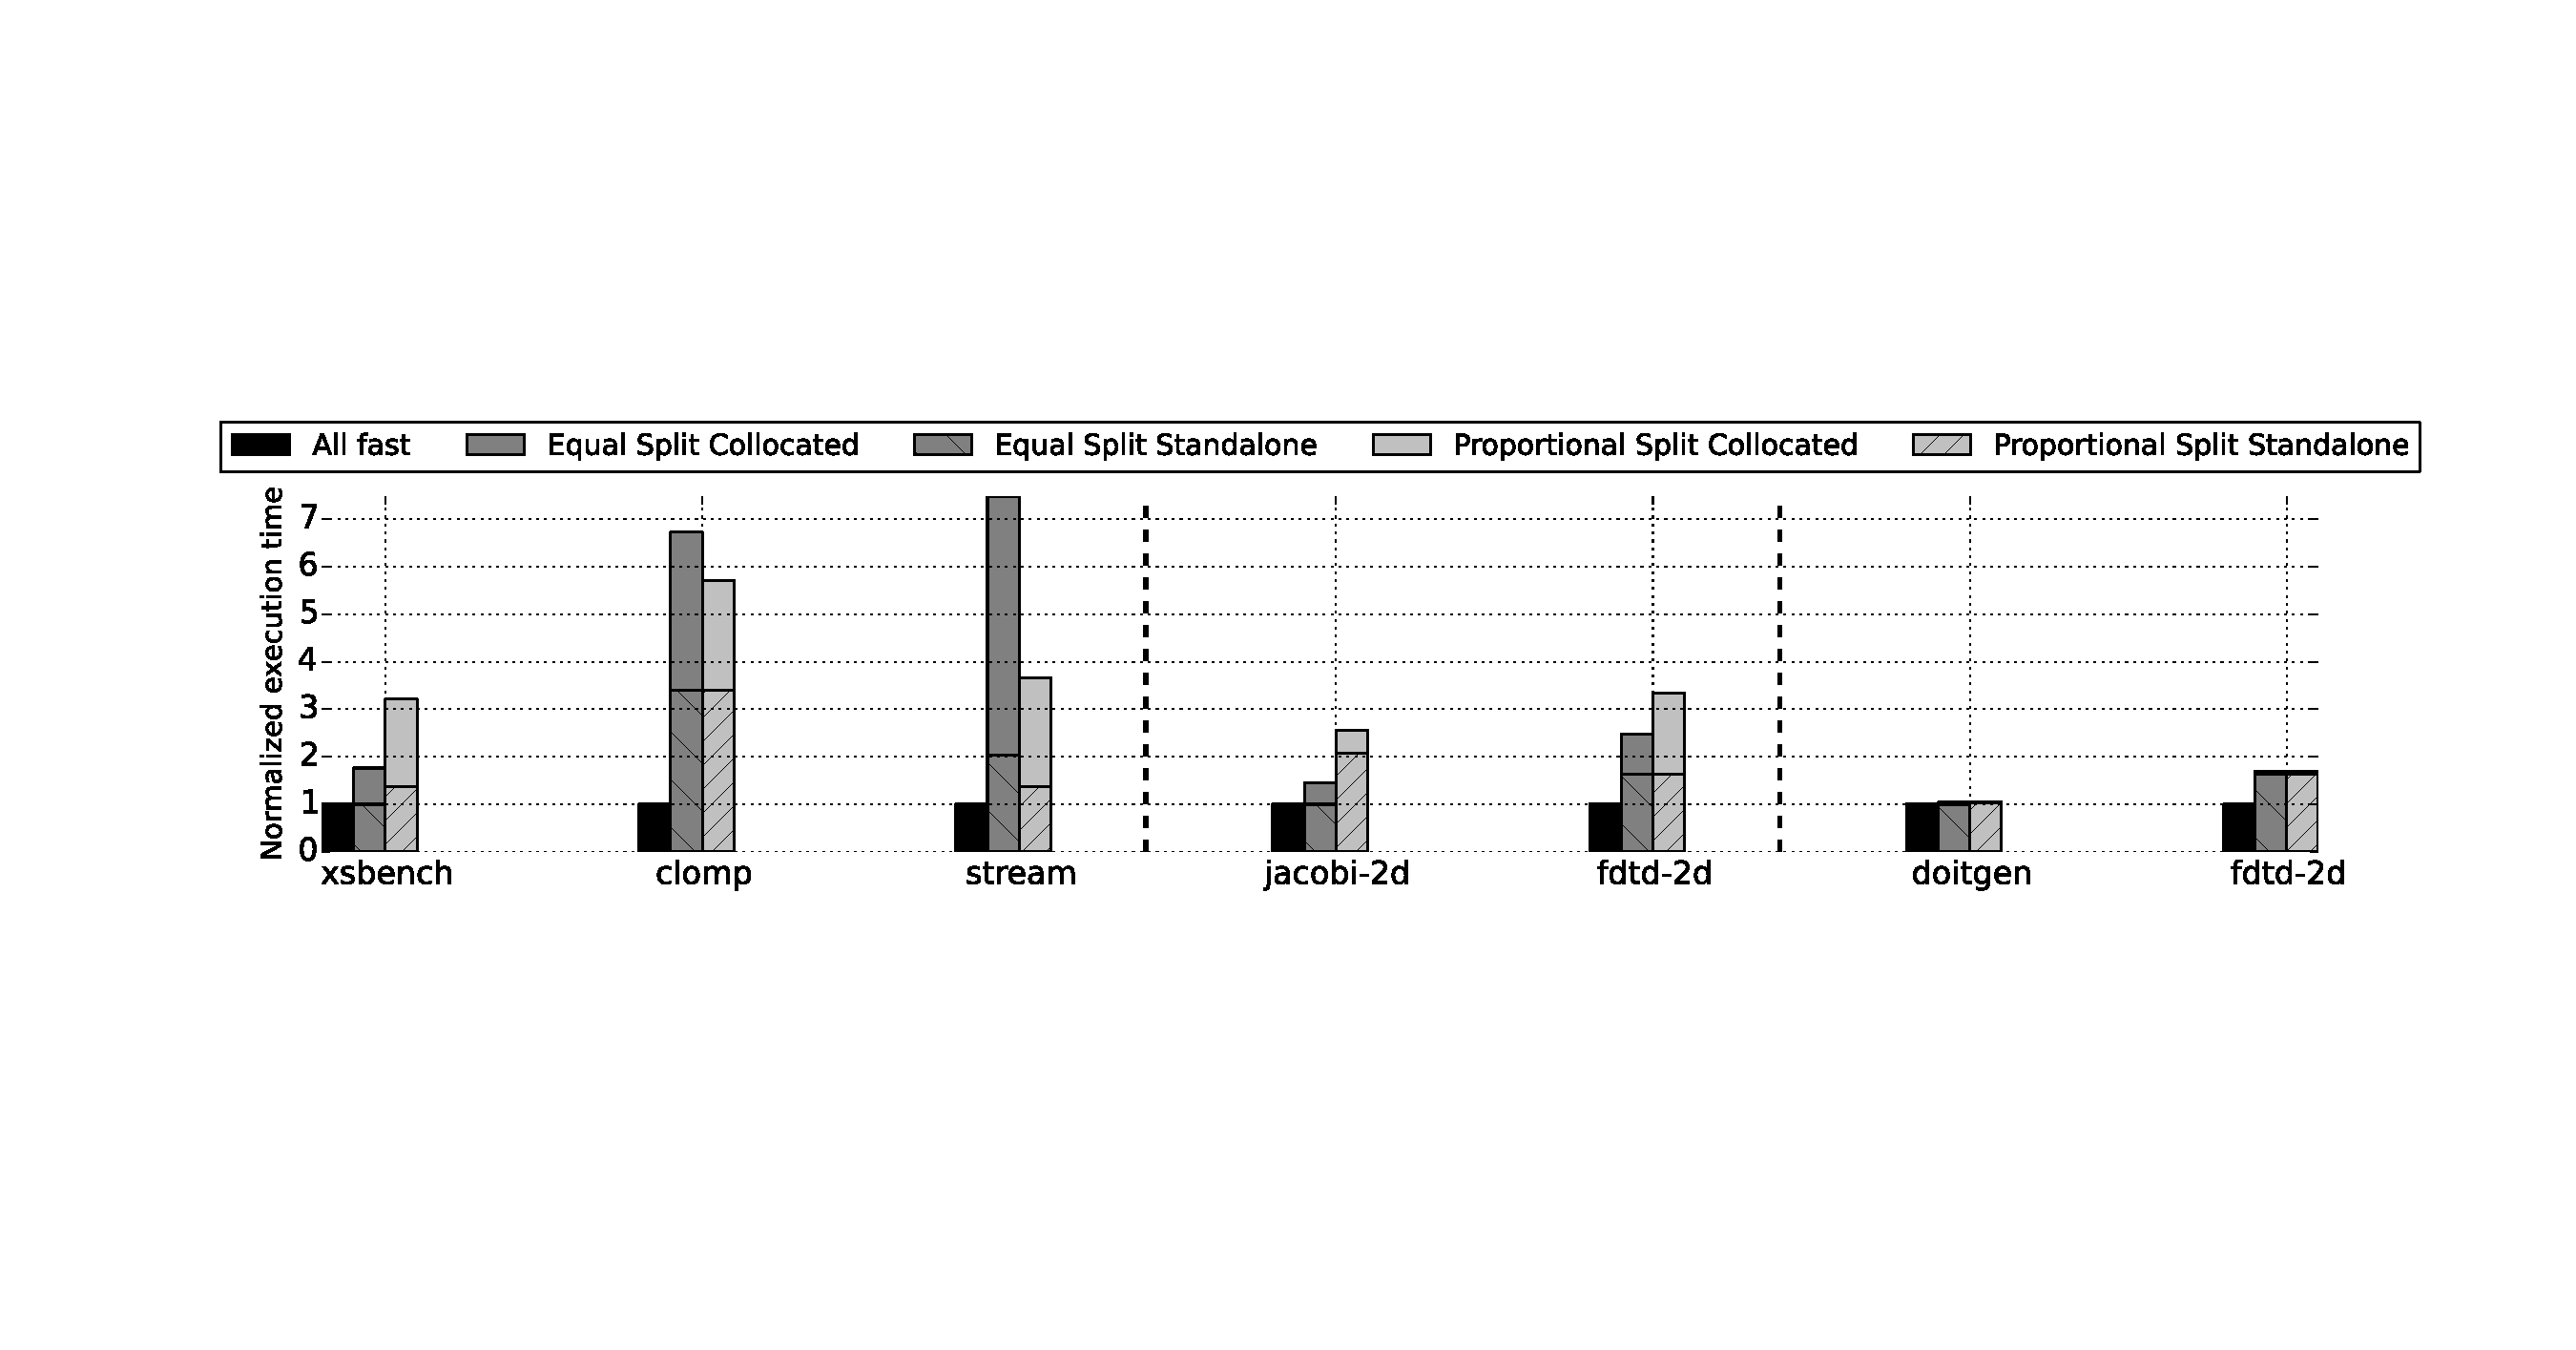
\includegraphics[width=\linewidth]{figures/tiering1.pdf}
      \captionsetup{labelformat=empty}
\caption{Execution time slowdown from `all-in-DRAM' for three different collocation combinations (separated with dashed lines). The shaded parts refer to the slowdown caused by data tiering. The unshaded parts depict the additional slowdown due to collocation. }
%  \label{fig:static}  
  \end{subfigure}

   \begin{subfigure}{\linewidth}
  \begin{subfigure}{0.425\linewidth}
  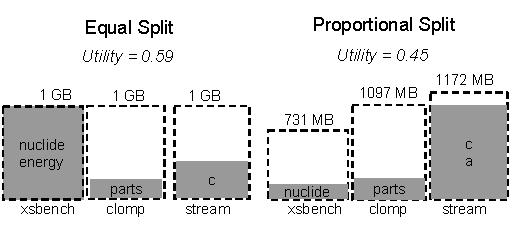
\includegraphics[width=\linewidth]{figures/tiering1a.pdf}
      \captionsetup{labelformat=empty}
  \caption{Collocation of XSBench, CLOMP, STREAM}
    \end{subfigure}%  
     \begin{subfigure}{0.3\linewidth}
  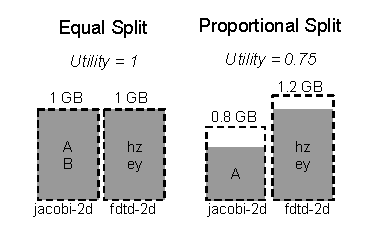
\includegraphics[width=\linewidth]{figures/tiering1b.pdf}
      \captionsetup{labelformat=empty}
    \caption{Collocation of jacobi-2d, fdtd-2d}
    \end{subfigure}%  
     \begin{subfigure}{0.3\linewidth}
     \centering
  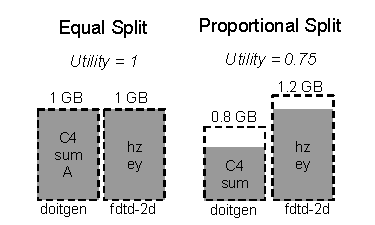
\includegraphics[width=\linewidth]{figures/tiering1c.pdf}
      \captionsetup{labelformat=empty}
    \caption{Collocation of doitgen, fdtd-2d}
    \end{subfigure}  
          \captionsetup{labelformat=empty}
  \caption{Utility and objects allocated in FastMem. The total available FastMem capacity is the sum of the private partitions of each application.}
  \end{subfigure}
  \caption{Comparison of equal and proportional capacity split schemas for three different collocation combinations.}
  \label{fig:tiering1}
    \vspace{-0.1in}
\end{figure*}

Data tiering techniques are able to mitigate the performance slowdown of an application, that spans its dataset across heterogeneous memory components, 
by occupying all the available FastMem and servicing with lower latency as many memory requests as possible. However, in the case of multi-tenant environments, the available FastMem will be yet another resource that needs to be fairly and optimally distributed across co-running applications.

In this section, we first experiment with techniques that divide the total available FastMem across the co-running kernels and evaluate their effectiveness. Then, based on the observations made in Section~\ref{sec:analysis}, regarding the sensitivity to slow memory on an application as well as data structure level, we further refine the tiering solutions for collocated workloads, proposing memory-sharing techniques. 

The performance of the proposed techniques across the CORAL and Polybench benchmarks is depicted in Figures~\ref{fig:tiering1},~\ref{fig:tiering2} and their effectiveness is  summarized in Table~\ref{tbl:tiering_summary} for the CORAL benchmarks.
We evaluate the effectiveness of all schemas, using the following criteria: 
\begin{tightenumerate}
\item The total runtime slowdown of an application when running in collocation, compared to standalone execution with all data allocated in FastMem (`All fast'). One part of this slowdown is attributed to SlowMem accesses due to data tiering and the other part captures the absolute impact of execution over shared resources. A technique that is able to highly mitigate this slowdown across most collocated applications is more efficient compared to the others.
\item The aggregate utilization of FastMem from all collocated applications. We define \(FastMem\ Utility = \frac{Bytes\ Allocated}{Capacity}\). Utility can be less than 1, if the workload size exceeds the FastMem capacity, due to the assumption that there is no support for partial object allocations, thus if a data structure doesn't fit into the available FastMem, it cannot be placed there, giving its position to the next object 
in the order determined by the benefit factors. High FastMem utility shows that the schema is able to make efficient use of the available FastMem and that will translate to higher application performance.\\
\end{tightenumerate}

\noindent All following techniques are static, because they assume that applications will first need to execute the offline profiling phase, that will determine the priority order for FastMem allocations of the different data objects, and then start execution using the part of FastMem they're entitled to. The partitioning schemas also require prior knowledge of the number of collocated applications, so as to define the amount of partitions. 

%%%%%%%%%%%%%%%%%%%%%%% Static Partitioning %%%%%%%%%%%%%%%%%%%%%%%%%%%%%%%%
\subsection{Static Partitioning}
\label{subsec:static}
Existing data tiering solutions, described in Section ~\ref{sec:intro},
can be directly applied into a shared heterogeneous memory system, when partitioning the available FastMem into parts private to each application. We experiment with the following predominant schemas to partition a shared resource.\\
\noindent{\bf Equal Capacity Split.}
This technique divides the available FastMem into parts that are equal for every application. More specifically, the available FastMem of total capacity C will be split into 
N parts of size $\frac{C}{N}$ for each out of the N workloads. It ensures fair partitioning of the available FastMem across the collocated applications. 

\noindent{\bf Propotional Capacity Split.}
This schema splits the available FastMem into parts that are proportional to the overall workload sizes. In more detail, if FastMem has total capacity C and 
each out of the N applications has size $S_i$, then FastMem will be divided into parts of size $C*\frac{S_i}{\sum_{i=1}^{N}S_i}$. This provides fairness on an application level and 
accounts for maximizing the FastMem utility, by adjusting the FastMem partitions to the application memory demands. \\

%\begin{table}[ht]
%\centering
%  \begin{tabular}{|p{1.2cm}||p{3cm}||p{3cm}|} \hline
%    Kernel & Equal split & Proportional Split \\\hline \hline
%    jacobi-2d 	& A (F) > B (F) &  A (F) > B (S) \\\hline
 %   fdtd-2d 	& hz (F) > ey (F) > ex (S) & hz (F) > ey (F) > ex (S) \\\hline
 %   doitgen 	& C4 (F) > sum (F) > A (F) & C4 (F) > sum (F) > A (S) \\\hline
 %   xsbench 	& nuclide (F) > energy (F) & nuclide (F) > energy (S) \\\hline
 %   clomp	 	& zones (S) > parts (F) & zones (S) > parts (F) \\\hline
%    stream 		& c (F) > a (S) > b (S) & c (F) > a (F) > b (S) \\\hline
 % \end{tabular}
%  \caption{Data tiering due to the capacity restrictions of the equal and proportional capacity split schemas. (F) indicates object allocation in FastMem, (S) in SlowMem.}
 % \label{tbl:tiering_split}
 % \vspace{-0.3in}
%\end{table}


%\subsubsection
\vspace{0.6ex}
\noindent{\bf\em CORAL Experiments}
\vspace{0.3ex} 

\noindent First, we experiment with three of the skeleton benchmarks in the CORAL suite. We collocate all three 
applications of 4.1 GB aggregate memory footprint, over 3 GB of shared FastMem and 4 GB of SlowMem.
The individual working set sizes are 1 GB for XSBench, 1.5 GB for CLOMP and 1.6 GB for STREAM, as shown in Table 
~\ref{tbl:tiering}. The partition sizes are 1 GB for each benchmark in the case of the equal capacity split method. 
For the proportional capacity split schema XSBench gets 731 MB of FastMem, CLOMP 1097 MB and STREAM 1172 MB. The objects allocated in FastMem for every collocated application are depicted in Figure ~\ref{fig:tiering1}. 
In addition, we run these three multi-threaded applications using 4 instead of 12 threads, so that when all three are 
co-executing they do not exceed the available cores on the node. In this way, we can eliminate other 
slowdown factors due to thread CPU scheduling and capture the overhead of sharing the hardware caches and 
memory subsystem. Furthermore, in order to account for the different run times of the three applications and 
the non-sensitive initialization phase of XSBench, we report the average run time of each one, excluding the very first and last run. Figure ~\ref{fig:tiering1} shows the slowdown of the applications due to data tiering and collocation.

First, we observe that XSBench runs faster in the equal capacity split schema, due to the fact that all of its dataset fits in FastMem. Additionally, in the case of the proportional capacity split, most of its slowdown comes from the collocation rather than the data tiering itself, due to the fact that the object that is now allocated in SlowMem, has trivial benefit factor. However, the allocation of the low benefit factor object of significant size (970 MB) in SlowMem, incurs up to 1.5x additional slowdown.

Second, although CLOMP has the same data tiering in both partitioning schemas, it gets to run faster in the case of proportional capacity split. This can most likely be	 attributed to the fact that there is extra bandwidth available to use from the SlowMem, due to the data tiering imposing more data allocations, thus accesses to FastMem, than in the equal capacity scplit.

Third, STREAM incurs bigger slowdown in the case of equal capacity split, due to the capacity restriction allowing to allocate only one object in FastMem. Also, most of its slowdown comes from collocation rather than data tiering, further highlighting the impact of SlowMem accesses in shared execution environments.

Finally, the equal capacity split schema accounts for 0.59 of FastMem utility, compared to 0.45 in the proportional capacity split. In both cases, the utility is very restricted and shows the limitation of partitioning techniques to make clever data placement decisions, something that is reflected in the significant application slowdown imposed by collocation for the given data tierings.
 
 \begin{table*}[t]
\centering
  \begin{tabular}{|p{1.5cm}|p{2cm}|p{9cm}|p{2.2cm}|p{1.2cm}|} \hline
	Category & Name & Technique & Slowdown from `all-in-FastMem' & FastMem utility    \\\hline \hline
    \multirow{2}{*}{Partitioning} & Equal Capacity Split & Creates equal partitions of FastMem across collocated kernels. Each kernel places objects to their partition, in descending benefit factor order.  & up to 7x & 0.59 \\\cline{2-5}
    & Proportional Capacity Split & Partitions FastMem in parts proportional to the individual workload sizes. Each kernel places objects to their partition, in descending benefit factor order. & up to 6x & 0.45\\\hline
        \multirow{3}{*}{Sharing} & Fair Merge & Places objects in FastMem following the descending benefit factor order, choosing from a different application at a time.  & up to 2.7x & 0.87\\\cline{2-5}
    & Blind Merge & Places objects in FastMem following the descending benefit factor absolute order of all applications. & up to 2.6x & 0.96 \\\cline{2-5}
    & {\bf CoMerge} & Places objects in FastMem following the descending {\it co-benefit factor} absolute order of all applications. Has the same effect with Blind Merge for kernels in the same sensitivity level. & up to 2.6x & 0.96 \\\hline
  \end{tabular}
  \caption{Summary and comparison of the effectiveness of data tiering techniques across the collocated CORAL benchmarks. Since these kernels belong to the same sensitivity level, Blind Merge and CoMerge have the same effect. Memory sharing techniques are efficient because they can significantly mitigate the runtime slowdown due to the higher FastMem utility.}
  \label{tbl:tiering_summary}
    \vspace{-0.3in}
\end{table*}


%\subsubsection
\vspace{2ex}
\noindent{\bf\em Polybench Experiments}
\vspace{0.3ex} 

\noindent Second, we experiment with collocating several Polybench kernels in pairs, two high sensitivity kernels jacobi-2d and fdtd-2d, as well as a high with a non sensitivite kernel fdtd-2d and doitgen. We fix the total available FastMem to be 2 GB. The working set sizes of the kernels are 1 GB for jacobi-2d and doitgen, and 1.5 GB for fdtd-2d, as you can refer back to Table ~\ref{tbl:tiering}. 
An equal capacity split schema will attribute 1 GB to each of the two co-running kernels. In contrast, a proportional capacity split schema will assign 0.8 GB of FastMem jacobi-2d and doitgen, 
and 1.2 GB of FastMem to fdtd-2d. Figure~\ref{fig:tiering1} shows the objects allocated in FastMem in both partitioning schemas. Figure ~\ref{fig:tiering1} also shows the execution time of each kernel for the two different collocation pairs, normalized to the baseline case where all data could fit into FastMem in standalone execution. 
Due to the different execution completion times of the kernels, we start them together, repeat them multiple times, and report the average run time, excluding the final run, when one kernel finished before the others.

First, we observe that data tiering itself impacts performance in the standalone execution, which is obvious in the case of the highly sensitive kernel jacobi-2d. However, this is not the case for the non sensitive kernel doitgen, where data tiering does not slowdown the execution time.
Second, the impact of collocation in both partitioning schemas is noticeable in the co-running execution of the high sensitivity kernels. Proportional capacity split provides slower runtime, due to the different data tiering of jacobi-2d, which influences fdtd-2d as well. However, we see that doitgen, which is a 
non-sensitive kernel, does not get impacted by data tiering, nor by collocation. More importantly, it does not affect the execution time of the collocated fdtd-2d, whose slowdown is attributed almost in total to data tiering. Finally, as far as the FastMem utility is concerned equal capacity split achieves full utilization due to the fact that the data structure sizes (500 MB) align well with the given capacity. This is not the case with proportional capacity split which utilizes FastMem by 0.75, because it tries to adjust to the overall workload size but fails to align well with the data structure sizes. \\

\noindent{\bf\em Takeaways}\\
\vspace{0.3ex}
\noindent Overall, this experiment first highlights the importance to identify the sensitivity level of a kernel, 
because non-sensitive ones can potentially co-exist with other applications without impacting their performance.  
Second, we identify the great contribution of collocation to the runtime slowdown and the fact that allocation in SlowMem of objects with low benefit factor can have a trivial impact on standalone execution, but a significant contribution to the overall application slowdown in shared execution environments. 
Third, we observe that static partitioning techniques, in general, can fail to provide high FastMem utility and hurt 
application performance if the combination of data object sizes and available capacity is not 
alligned and there is no OS-level support for finer granularity data allocations. Thus, even though these techniques provide fairness in the use of FastMem, they may end up hurting not only the individual application performance, but also the performance of the collocated ones. 
 
%%%%%%%%%%%%%%%%%%%%%%% Sharing policy %%%%%%%%%%%%%%%%%%%%%%%%%%%%%%%% 
 
\subsection{Sharing policies}
\label{subsec:merge}

\begin{figure*}
  \centering
\begin{subfigure}{\linewidth}
  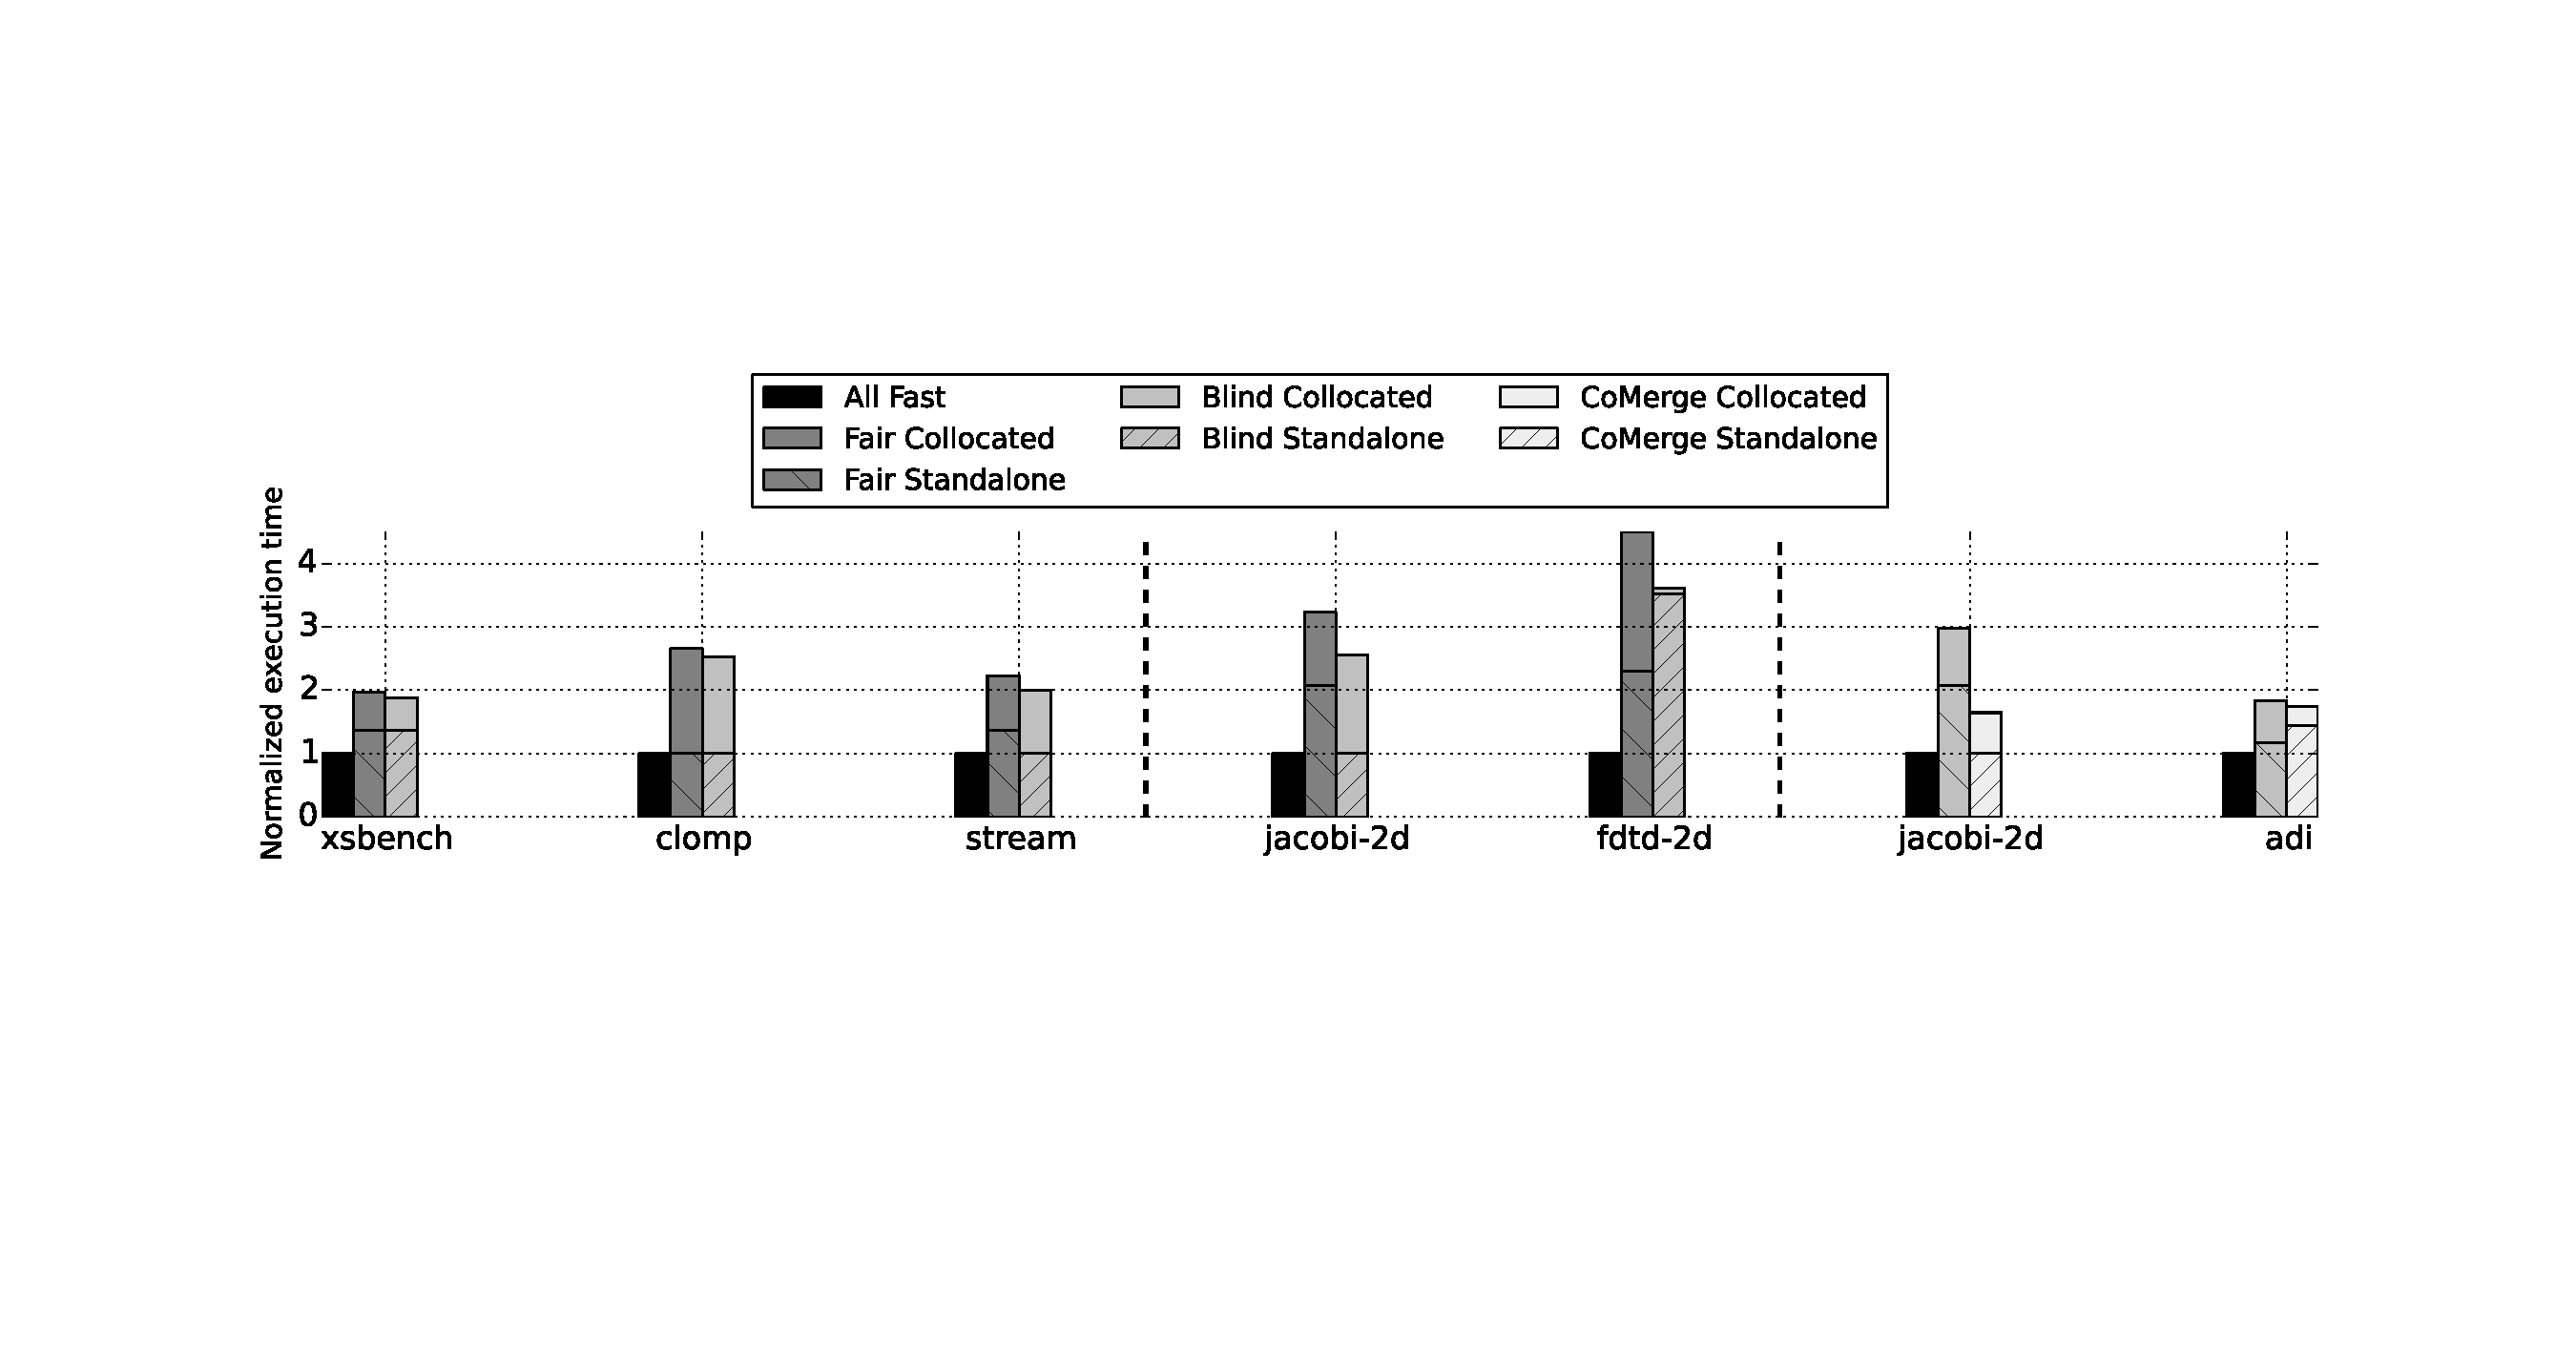
\includegraphics[width=\linewidth]{figures/tiering2.pdf}

      \captionsetup{labelformat=empty}

\caption{Execution time slowdown from `all-in-DRAM' for three different collocation combinations (separated with dashed lines). The shaded parts refer to the slowdown caused by data tiering. The unshaded parts depict the additional slowdown due to collocation.}
%  \label{fig:static}  
  \end{subfigure}

\begin{subfigure}{\linewidth}
  \begin{subfigure}{0.425\linewidth}
  	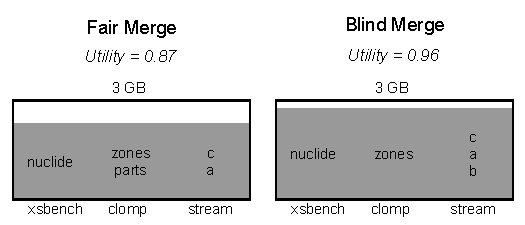
\includegraphics[width=\linewidth]{figures/tiering2a.pdf}
      \captionsetup{labelformat=empty}
  	\caption{Collocation of XSBench, CLOMP, STREAM}
  \end{subfigure}%  
     \begin{subfigure}{0.3\linewidth}
  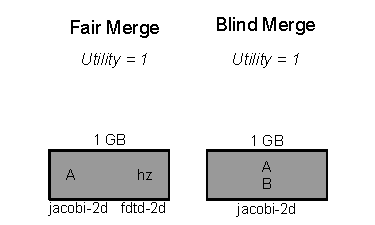
\includegraphics[width=\linewidth]{figures/tiering2b.pdf}
      \captionsetup{labelformat=empty}
    \caption{Collocation of jacobi-2d, fdtd-2d}
    \end{subfigure}%  
     \begin{subfigure}{0.3\linewidth}
     \centering
  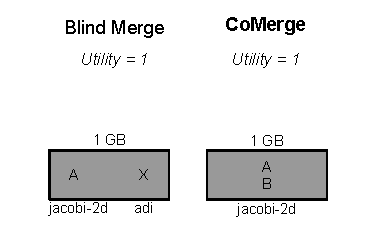
\includegraphics[width=\linewidth]{figures/tiering2c.pdf}
      \captionsetup{labelformat=empty}
    \caption{Collocation of jacobi-2d, adi}
    \end{subfigure}  
          \captionsetup{labelformat=empty}
  \caption{Utility and objects allocated in FastMem. }
  \end{subfigure}
  \caption{Comparison of Fair Merge, Blind Merge and CoMerge schemas for three different collocation combinations.}
    \label{fig:tiering2}

    \vspace{-0.1in}



\end{figure*}

Static partitioning techniques are essentially just applying the data tiering solutions to environments with even more restricted capacity. Especially in cases with very limited FastMem capacity, each placement decision can be crucial. 
In this section, we leverage the fact that the benefit factor values provide a normalized metric that captures the impact of the different application data structures on the overall workload sensitivity to execution over slower memory. We explore memory sharing schemas, so as to maximize the overall FastMem utility and facilitate decisions that increase performance across all applications, even if that restricts the fair usage of the shared FastMem.	
The following sharing policies merge the data structures of all collocated applications into a global object pool, where each object can be identified by the application where it belongs, its size and its benefit factor value. Then, they place objects into FastMem in descending order of benefit factor value, until total FastMem capacity is full. This is essentially a greedy algorithm, 
that can have two variances. \\

\noindent{\bf Fair merge.} This technique orders the objects of all collocated applications by merging them in descending benefit factor order and choosing from a different workload each time.
This schema ensures fairness, because it guarantees that all applications will be able to allocate part of their dataset in FastMem, if there is enough available capacity. It is susceptible to unfair cases, though, where 
an application with one object of significant size and high benefit factor, may take up the majority of the available FastMem space. Also, the application order of choice impacts the data tiering, as there may be cases where some applications may have more objects in FastMem than others. We define this order with respect to the overall dataset size, so as to prioritize applications with bigger memory footprint. \\
\noindent{\bf Blind merge.} This is a direct mergesort of the actual benefit factor values of the different data objects across the co-existing kernels, ignoring any application order. It allows for possible scenarios where one application may get full priority over another one, 
because its objects have bigger benefit factor values than the objects of the other kernels.\\

\begin{comment}
\begin{table}[t]
\centering
  \begin{tabular}{|p{1.2cm}||p{3cm}||p{3cm}|} \hline
    Kernel & Fair merge & Blind merge \\\hline \hline
    jacobi-2d 	& A (F) > B (S) &  A (F) > B (F) \\\hline
    fdtd-2d 	& hz (F) > ey (S) > ex (S) & hz (S) > ey (S) > ex (S) \\\hline
        xsbench 	& nuclide (F) > energy (S) & nuclide (F) > energy (S) \\\hline
    clomp	 	& zones (F) > parts (F) & zones (F) > parts (S) \\\hline
    stream 		& c (F) > a (F) > b (S) & c (F) > a (F) > b (F) \\\hline
  \end{tabular}
  \caption{Data tiering due to the capacity restrictions over fair and blind merge schemas. (F) indicates object allocation in FastMem, (S) in SlowMem.}
  \label{tbl:tiering_merge}
    %\vspace{-0.3in}
\end{table}
\end{comment}

%\begin{figure}[t]
  %\centering
%  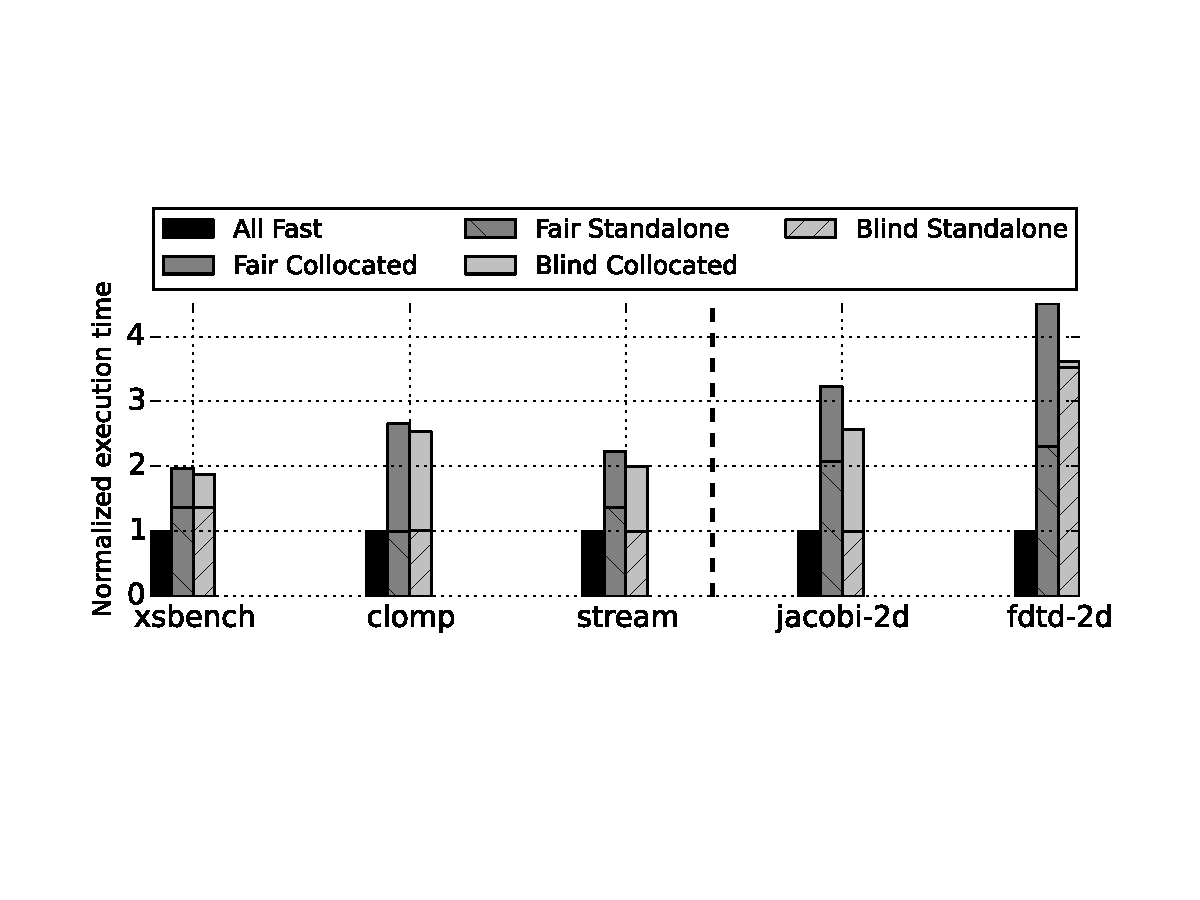
\includegraphics[width=\columnwidth]{figures/merge.pdf}
  %\caption{Execution time slowdown from 'all-in-FastMem' for the fair and blind merge schemas and two different collocation scenarios. The shaded parts refer to the slowdown caused by data tiering. The unshaded parts depict the additional slowdown due to collocation.}
  %\label{fig:merge}
%    \vspace{-0.3in}
%\end{figure}

%\subsubsection
\vspace{1ex}
\noindent{\bf\em CORAL Experiments}
\vspace{0.3ex} 

\noindent First, we experiment using the CORAL benchmarks configuration as in the previous subsection. The aggregate memory footprint is 4.1 GB and the available FastMem is 3 GB. The application data structures now form a global object pool whose sizes and benefit factor values are listed in table~\ref{tbl:tiering}. In the fair merge schema, we choose one object at a time from every application, in descending order of overall dataset size. Thus, we choose one object from STREAM, then CLOMP and then XSBench and repeat until FastMem cannot fit any other whole objects. The objects allocated in FastMem are depicted in Figure~\ref{fig:tiering2}. Similarly, for the blind merge schema we sort all objects from the global pool, in descending absolute benefit factor value and place them in FastMem until no other object fits. 
Figure~\ref{fig:tiering2} also shows the execution time slowdown of each collocated application due to data tiering and collocation.

To begin with, as far as the slowdown due to data tiering is concerned, we see that it is similar in both fair and blind merge schemas. This is due to the fact that XSBench has the same data tiering, whereas CLOMP has a trivial benefit factor object in SlowMem and STREAM has all of its dataset in FastMem in the blind merge schema. 
Second, regarding the slowdown due to collocation we see that all applications benefit from the blind merge schema. This schema enables the optimal global data placement, because it keeps in FastMem the objects from XSBench and CLOMP that have a really high benefit factor and allocates all the dataset of STREAM in FastMem. This global data tiering, allows applications to benefit both from low access times to the objects that are critical to performance and allocated in FastMem. Additionally, it maintains the low impact to performance of the objects with low benefit factor, due to the efficient utilization of the SlowMem bandwidth. This was not the case in the static partitioning schemas, where objects with low benefit factor that were allocated in SlowMem would impact significantly the collocation slowdown, due to their accesses being interleaved with objects of high benefit factor allocated in SlowMem, inflicted by the un-intelligent data tiering imposed by the partitioning schema. Finally, we observe that the blind merge schema allows almost optimal FastMem utility of 0.96, compared to 0.87 with the fair merge schema. 

Overall, the blind merge schema facilitates an optimal global data placement across co-running applications and high FastMem utility, leveraging the low access time for objects in FastMem with high benefit factor, as well as maintaining the low impact to performance slowdown of objects with low benefit factor, due to the efficient usage of the SlowMem bandwidth.\\

\vspace{1.5ex}
\noindent{\bf\em Polybench Experiments}
\vspace{0.3ex} 

\noindent We now experiment with a setup where the overall FastMem capacity is 1 GB, so as to highlight the importance of each individual choice in an environment with restricted FastMem capacity. We collocate 
two high sensitivity kernels jacobi-2d and fdtd-2d, which have data objects of 500 MB each. Figure~\ref{fig:tiering2} shows the tiering when applying fair and blind merge. 
More specifically, fair merge will choose the object with highest benefit factor from each application. In contrast, blind merge prioritizes jacobi-2d over fdtd-2d, because its data objects have 
higher overall benefit factor values, as you can refer back to table ~\ref{tbl:tiering}. Figure ~\ref{fig:tiering2} shows the execution time of each collocated kernel, normalized to the baseline case where all data could fit into FastMem in 
standalone execution. 
We can first observe the impact of data tiering, especially in the case of fdtd-2d, where blind merge is equivalent to the worst case scenario, where all objects are allocated in SlowMem. 
However, we notice that blind merge leads to less overall slowdown during collocation. This can be potentially attributed to the fact that memory requests can be serviced in parallel from FastMem and SlowMem for the different applications due to the better bandwidth usage distribution, even 
though accessing SlowMem maybe incur higher latency. Overall, prioritizing one application over another one, even though it's not fair, it may lead to better performance across both applications. 


\begin{comment}
\begin{table}[t]
\centering
  \begin{tabular}{|p{1.2cm}||p{3cm}||p{3cm}|} \hline
    Kernel & Blind merge & Blind co-merge \\\hline \hline
    jacobi-2d 	& A (F) > B (S) &  A (F) > B (F) \\\hline
    adi 	& X (F) > B (S) > A (S) & X (S) > B (S) > A (S) \\\hline
  \end{tabular}
  \caption{Data tiering due to the capacity restrictions over blind merge and co-merge schemas. (F) indicates object allocation in FastMem, (S) in SlowMem.}
  \label{tbl:co-merge}
     %\vspace{-0.3in}
\end{table}
\end{comment}

%\begin{figure}[t]
  %\centering
  %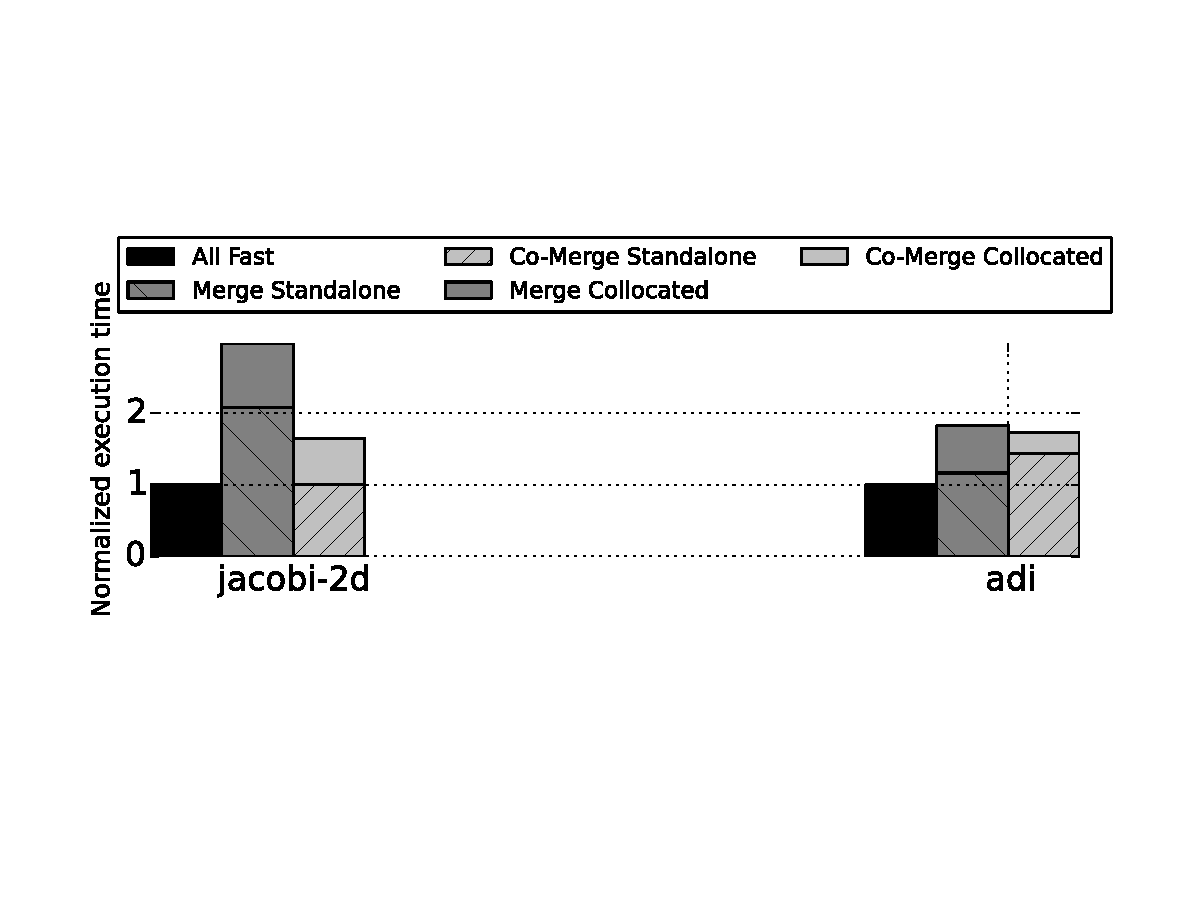
\includegraphics[width=\columnwidth]{figures/comerge.pdf}
%  \caption{Execution time slowdown from 'all-in-FastMem' for the blind merge and co-merge schemas. 
  %The shaded parts refer to the slowdown caused by data tiering. The unshaded parts depict the additional slowdown due to collocation.}
  %\label{fig:co-merge}
    %  \vspace{-0.3in}
%\end{figure}

We now apply the blind merge schema, when collocating high and low sensitivity kernels, jacobi-2d and adi.  We observe in Figure~\ref{fig:tiering2} that for the blind merge schema, the impact of collocation compared to standalone and baseline, is much more significant for jacobi-2d as it is a high sensitivity kernel, 
rather than adi that has very low sensitivity. Therefore, we see that jacobi-2d is in greater need of FastMem, so as to mitigate the performace slowdown. 
However, the absolute benefit factor values do not capture the overall sensitivity of the application. This is the reason why, we propose a {\it co-benefit factor}, which scales the current benefit factor by a value that 
corresponds to the overall slowdown of the application execution time when all data is allocated in SlowMem compared to FastMem, which is the value that essentially captures the overall application sensitivity level. 
\[Co-Benefit(O) = floor(\frac{S}{F})*\frac{t(O)-S}{F-S}\]
Table~\ref{tbl:tiering} includes the co-benefit values for the different objects of every application. We note that non-sensitive kernels have zero co-benefit values, because they should not get prioritized for placement in FastMem, 
as allocation in SlowMem does not impact overall performace. \\

\noindent{\bf CoMerge.} This is a direct mergesort of the {\it co-benefit factor} values of the data structures across all collocated applications. Objects are placed in FastMem in descending co-benefit factor order, until no other object can be placed due to capacity restrictions. 
Since the co-benefit factor now captures the overall application sensitivity to SlowMem, objects from more sensitive workloads get higher weight thus priority in the above sorting.
 If the collocated applications belong in the same sensitivity level, then the technique is the same with the blind merge, due to the way the co-benefit factor is calculated to scale with the level of sensitivity. 
 
Therefore, back in the example of Figure~\ref{fig:tiering2} we see that a CoMerge policy will prioritize jacobi-2d over adi and this data arrangement mitigates the 
slowdown for both kernels, even more significantly for jacobi-2d that is a high sensitivity kernel. \\

\vspace{0.8ex}
\noindent{\bf\em Takeaways}
\vspace{0.3ex} 

\noindent In conclusion, we propose CoMerge, a memory sharing technique that can provide the most intelligent global data tiering of application data structures that are collocated in shared heterogeneous memory environments. First, CoMerge is able to maximize the FastMem utility due to the fact that is a memory sharing technique. Second, it can efficiently mitigate the performance slowdown across all collocated applications, via the use of co-benefit factor values that are able to capture the exact impact of a data structure to the application performance in shared environments, incorporating the overall application sensitivity to SlowMem. CoMerge sorts the global object pool in descending co-benefit factor value and allocates them in FastMem until capacity is full. This technique leverages both the fast access time to FastMem for objects with high benefit factor, as well as the  SlowMem bandwidth for objects with low benefit factor. 


\section{Future Work}

Moving forward, there is great need to diverge from a-priori offline profiling solutions. CoMerge can function under the assumption that 
applications are profiled and the global tiering is determined, before they can all start executing. This is not the case in the majority of multi-tenant environments, where different users can share resources and 
execute dynamic workloads at any point of time. Thus, offline profiling and synchronized solutions are very restrictive. This observation further enhances the need for OS-level online solutions, that need to monitor the behavior of 
applications, focusing on the data structures that are critical to performance, in order to determine sensitivity levels and migrations decisions, so as to maximize the utility and fairly resolve the competition for fast memory allocations 
across different co-existing kernels. We believe that there can be cross-stack solutions, where application hints or compliler-assisted solutions can help identify the critical to performance data structures and limit the 
spectrum of the unavoidable OS-level online monitoring infrastructure. 
\section{Summary}
\begin{comment}
In this work we investigate the need for new tools and policies that can efficiently span and cleverly map application's data 
across a heterogenous memory substrate. 
Existing solutions rely on detailed offline profiling of applications' data structures and associated access behaviors, and calculate costs that establish a priority 
with which a memory object should be allocated in the available FastMem during the online run. However, these tools make the 
assumption that an application is static and that it can use all the available FastMem.  %which is not the case for applications with dynamic, input-dependent behaviors, or in shared multi-tenant environments.  
Consequently, the current approaches are limited in their ability to support complex applications with dynamic data-dependent 
behaviors, or to be used in shared multi-tenant environments. 
 %Also, they rely on application-level hints as input. 
Ideally, we would like to have system-level support, that can on-the-fly 
decide the best data placement, as well as migrate memory objects either when the application itself changes a phase, or when 
other co-located applications demand to use more of certain memory component. Although there is such support in NUMA systems, 
these policies are shown not be effective in hybrid memory systems with much larger degree of variability in latency, bandwidth and capacity characteristics~\cite{sudarsun:isca17,bonnie}. 

Our observations after extensive analysis of a representative benchmark suite of the HPC domain, show that there is potential to 
simplify the existing approaches, so that they can more easily be integrated in dynamic system-level solution. More specifically, we 
first notice than not all applications are sensitive to memory heterogeneity and second not all application's data 
structures increase performance when placed in FastMem. Therefore, we propose that we need to shift the efforts from 
calculating an ordering of the data structures, to determining which ones are critical to performance. In this way, 
if we can quickly identify the benefit an application overall or some of its data objects have from FastMem allocation, 
we can significantly reduce the overhead and metadata needed to make online decisions about placement and migrations. 
For example, in most kernels the data structure that was holding the input data and used in computation, was usually the one 
that incurred almost 0.9 benefit from being placed in FastMem, due to the significant size and number of accesses received, 
compared to the rest.  Therefore, as HPC expert programmers and compiler tools try to build cache-friendly access patterns with techniques 
like dependency analysis and loop unrolling, they could similarly identify such key data structures and forward placement hints to the system-level managers. 

In particular, a system-level solution for dynamic placement and migration of application data should be able to quickly 
classify if a data object or application overall is sensitive to memory heterogeneity or not. This has a threefold importance. 
First, it will reduce the complexity of the framework as it can restrict tracking to only the absolutely necessary memory regions, 
providing a simpler and possibly faster solution. Second, it can actually leverage the use of SlowMem and not treat it as a 
last option due to the restricted capacity of FastMem, and thus improve overall system cost and efficiency metrics. Finally, the use of a characterization metric such as ``benefit factor'', which normalizes the data structure's 
or memory region's contribution to sensitivity, can present an opportunity for establishing fairness or SLA guarantees in multi-tenant 
environments, where all applications will compete for FastMem, thus requiring policies for FastMem partitioning and data migration.  
%, thus there needs to be a policy that will monitor the 
%partition of FastMem and respectively migrate data when it is required.
\end{comment}

In this work we investigate the potential to extend existing data tiering solutions, in order to facilitate efficient data placement and mitigate the performance slowdown across applications in shared heterogenous memory subsytems.
We propose {\it CoMerge}, a memory-sharing schema that merges per application tierings and a-priori decides the priority placements across applications, with respect to the overall application sensitivity to accesses in slower memory components 
and the available fast memory capacity. We motivate the need for sensitivity aware decisions, based on the observations that applications or application phases may incur different degrees of slowdown when allocating data in slow memory, as well as the 
fact that not all applications' data structures contribute equally to the overall execution time. This applies for both single as well multi-threaded applications. We define a per data object {\it co-benefit factor}, which captures the importance of allocating the object in FastMem by observing its contribution to the workload runtime with respect to the overall application sensitivity to slower memory.
We first experiment with static partitioning schemas, and show that they may fail to maximize the utilization 
of the available fast memory as well as significantly hurt performance due to un-intelligent data tiering. Then, we show that with CoMerge, a memory sharing policy, we can achieve optimal data tiering across all collocated applications via ordering fast memory allocations according to the object's co-benefit factor. In this way, we achieve high utilization of the shared fast memory and mitigate the slowdown across all collocated applications, even though fairly distributed usage of the fast memory is not guaranteed.\\

\noindent{\bf Acknowledgement. } We thank the anonymous reviewers for their helpful feedback. This work is supported by the Department of Energy, through the ECP SICM and SSIO UNITY projects.


\bibliographystyle{ACM-Reference-Format}
\bibliography{memspan}

\end{document}
